%%%%%%%% ICML 2026 EXAMPLE LATEX SUBMISSION FILE %%%%%%%%%%%%%%%%%

\documentclass{article}

% Optional math commands from https://github.com/goodfeli/dlbook_notation.
%%%%% NEW MATH DEFINITIONS %%%%%

\usepackage{amsmath,amsfonts,bm}

% Mark sections of captions for referring to divisions of figures
\newcommand{\figleft}{{\em (Left)}}
\newcommand{\figcenter}{{\em (Center)}}
\newcommand{\figright}{{\em (Right)}}
\newcommand{\figtop}{{\em (Top)}}
\newcommand{\figbottom}{{\em (Bottom)}}
\newcommand{\captiona}{{\em (a)}}
\newcommand{\captionb}{{\em (b)}}
\newcommand{\captionc}{{\em (c)}}
\newcommand{\captiond}{{\em (d)}}

% Highlight a newly defined term
\newcommand{\newterm}[1]{{\bf #1}}


% Figure reference, lower-case.
\def\figref#1{figure~\ref{#1}}
% Figure reference, capital. For start of sentence
\def\Figref#1{Figure~\ref{#1}}
\def\twofigref#1#2{figures \ref{#1} and \ref{#2}}
\def\quadfigref#1#2#3#4{figures \ref{#1}, \ref{#2}, \ref{#3} and \ref{#4}}
% Section reference, lower-case.
\def\secref#1{section~\ref{#1}}
% Section reference, capital.
\def\Secref#1{Section~\ref{#1}}
% Reference to two sections.
\def\twosecrefs#1#2{sections \ref{#1} and \ref{#2}}
% Reference to three sections.
\def\secrefs#1#2#3{sections \ref{#1}, \ref{#2} and \ref{#3}}
% Reference to an equation, lower-case.
\def\eqref#1{equation~\ref{#1}}
% Reference to an equation, upper case
\def\Eqref#1{Equation~\ref{#1}}
% A raw reference to an equation---avoid using if possible
\def\plaineqref#1{\ref{#1}}
% Reference to a chapter, lower-case.
\def\chapref#1{chapter~\ref{#1}}
% Reference to an equation, upper case.
\def\Chapref#1{Chapter~\ref{#1}}
% Reference to a range of chapters
\def\rangechapref#1#2{chapters\ref{#1}--\ref{#2}}
% Reference to an algorithm, lower-case.
\def\algref#1{algorithm~\ref{#1}}
% Reference to an algorithm, upper case.
\def\Algref#1{Algorithm~\ref{#1}}
\def\twoalgref#1#2{algorithms \ref{#1} and \ref{#2}}
\def\Twoalgref#1#2{Algorithms \ref{#1} and \ref{#2}}
% Reference to a part, lower case
\def\partref#1{part~\ref{#1}}
% Reference to a part, upper case
\def\Partref#1{Part~\ref{#1}}
\def\twopartref#1#2{parts \ref{#1} and \ref{#2}}

\def\ceil#1{\lceil #1 \rceil}
\def\floor#1{\lfloor #1 \rfloor}
\def\1{\bm{1}}
\newcommand{\train}{\mathcal{D}}
\newcommand{\valid}{\mathcal{D_{\mathrm{valid}}}}
\newcommand{\test}{\mathcal{D_{\mathrm{test}}}}

\def\eps{{\epsilon}}


% Random variables
\def\reta{{\textnormal{$\eta$}}}
\def\ra{{\textnormal{a}}}
\def\rb{{\textnormal{b}}}
\def\rc{{\textnormal{c}}}
\def\rd{{\textnormal{d}}}
\def\re{{\textnormal{e}}}
\def\rf{{\textnormal{f}}}
\def\rg{{\textnormal{g}}}
\def\rh{{\textnormal{h}}}
\def\ri{{\textnormal{i}}}
\def\rj{{\textnormal{j}}}
\def\rk{{\textnormal{k}}}
\def\rl{{\textnormal{l}}}
% rm is already a command, just don't name any random variables m
\def\rn{{\textnormal{n}}}
\def\ro{{\textnormal{o}}}
\def\rp{{\textnormal{p}}}
\def\rq{{\textnormal{q}}}
\def\rr{{\textnormal{r}}}
\def\rs{{\textnormal{s}}}
\def\rt{{\textnormal{t}}}
\def\ru{{\textnormal{u}}}
\def\rv{{\textnormal{v}}}
\def\rw{{\textnormal{w}}}
\def\rx{{\textnormal{x}}}
\def\ry{{\textnormal{y}}}
\def\rz{{\textnormal{z}}}

% Random vectors
\def\rvepsilon{{\mathbf{\epsilon}}}
\def\rvtheta{{\mathbf{\theta}}}
\def\rva{{\mathbf{a}}}
\def\rvb{{\mathbf{b}}}
\def\rvc{{\mathbf{c}}}
\def\rvd{{\mathbf{d}}}
\def\rve{{\mathbf{e}}}
\def\rvf{{\mathbf{f}}}
\def\rvg{{\mathbf{g}}}
\def\rvh{{\mathbf{h}}}
\def\rvu{{\mathbf{i}}}
\def\rvj{{\mathbf{j}}}
\def\rvk{{\mathbf{k}}}
\def\rvl{{\mathbf{l}}}
\def\rvm{{\mathbf{m}}}
\def\rvn{{\mathbf{n}}}
\def\rvo{{\mathbf{o}}}
\def\rvp{{\mathbf{p}}}
\def\rvq{{\mathbf{q}}}
\def\rvr{{\mathbf{r}}}
\def\rvs{{\mathbf{s}}}
\def\rvt{{\mathbf{t}}}
\def\rvu{{\mathbf{u}}}
\def\rvv{{\mathbf{v}}}
\def\rvw{{\mathbf{w}}}
\def\rvx{{\mathbf{x}}}
\def\rvy{{\mathbf{y}}}
\def\rvz{{\mathbf{z}}}

% Elements of random vectors
\def\erva{{\textnormal{a}}}
\def\ervb{{\textnormal{b}}}
\def\ervc{{\textnormal{c}}}
\def\ervd{{\textnormal{d}}}
\def\erve{{\textnormal{e}}}
\def\ervf{{\textnormal{f}}}
\def\ervg{{\textnormal{g}}}
\def\ervh{{\textnormal{h}}}
\def\ervi{{\textnormal{i}}}
\def\ervj{{\textnormal{j}}}
\def\ervk{{\textnormal{k}}}
\def\ervl{{\textnormal{l}}}
\def\ervm{{\textnormal{m}}}
\def\ervn{{\textnormal{n}}}
\def\ervo{{\textnormal{o}}}
\def\ervp{{\textnormal{p}}}
\def\ervq{{\textnormal{q}}}
\def\ervr{{\textnormal{r}}}
\def\ervs{{\textnormal{s}}}
\def\ervt{{\textnormal{t}}}
\def\ervu{{\textnormal{u}}}
\def\ervv{{\textnormal{v}}}
\def\ervw{{\textnormal{w}}}
\def\ervx{{\textnormal{x}}}
\def\ervy{{\textnormal{y}}}
\def\ervz{{\textnormal{z}}}

% Random matrices
\def\rmA{{\mathbf{A}}}
\def\rmB{{\mathbf{B}}}
\def\rmC{{\mathbf{C}}}
\def\rmD{{\mathbf{D}}}
\def\rmE{{\mathbf{E}}}
\def\rmF{{\mathbf{F}}}
\def\rmG{{\mathbf{G}}}
\def\rmH{{\mathbf{H}}}
\def\rmI{{\mathbf{I}}}
\def\rmJ{{\mathbf{J}}}
\def\rmK{{\mathbf{K}}}
\def\rmL{{\mathbf{L}}}
\def\rmM{{\mathbf{M}}}
\def\rmN{{\mathbf{N}}}
\def\rmO{{\mathbf{O}}}
\def\rmP{{\mathbf{P}}}
\def\rmQ{{\mathbf{Q}}}
\def\rmR{{\mathbf{R}}}
\def\rmS{{\mathbf{S}}}
\def\rmT{{\mathbf{T}}}
\def\rmU{{\mathbf{U}}}
\def\rmV{{\mathbf{V}}}
\def\rmW{{\mathbf{W}}}
\def\rmX{{\mathbf{X}}}
\def\rmY{{\mathbf{Y}}}
\def\rmZ{{\mathbf{Z}}}

% Elements of random matrices
\def\ermA{{\textnormal{A}}}
\def\ermB{{\textnormal{B}}}
\def\ermC{{\textnormal{C}}}
\def\ermD{{\textnormal{D}}}
\def\ermE{{\textnormal{E}}}
\def\ermF{{\textnormal{F}}}
\def\ermG{{\textnormal{G}}}
\def\ermH{{\textnormal{H}}}
\def\ermI{{\textnormal{I}}}
\def\ermJ{{\textnormal{J}}}
\def\ermK{{\textnormal{K}}}
\def\ermL{{\textnormal{L}}}
\def\ermM{{\textnormal{M}}}
\def\ermN{{\textnormal{N}}}
\def\ermO{{\textnormal{O}}}
\def\ermP{{\textnormal{P}}}
\def\ermQ{{\textnormal{Q}}}
\def\ermR{{\textnormal{R}}}
\def\ermS{{\textnormal{S}}}
\def\ermT{{\textnormal{T}}}
\def\ermU{{\textnormal{U}}}
\def\ermV{{\textnormal{V}}}
\def\ermW{{\textnormal{W}}}
\def\ermX{{\textnormal{X}}}
\def\ermY{{\textnormal{Y}}}
\def\ermZ{{\textnormal{Z}}}

% Vectors
\def\vzero{{\bm{0}}}
\def\vone{{\bm{1}}}
\def\vmu{{\bm{\mu}}}
\def\vsigma{{\bm{\sigma}}}
\def\veta{{\bm{\eta}}}
\def\vtheta{{\bm{\theta}}}
\def\va{{\bm{a}}}
\def\vb{{\bm{b}}}
\def\vc{{\bm{c}}}
\def\vd{{\bm{d}}}
\def\ve{{\bm{e}}}
\def\vf{{\bm{f}}}
\def\vg{{\bm{g}}}
\def\vh{{\bm{h}}}
\def\vi{{\bm{i}}}
\def\vj{{\bm{j}}}
\def\vk{{\bm{k}}}
\def\vl{{\bm{l}}}
\def\vm{{\bm{m}}}
\def\vn{{\bm{n}}}
\def\vo{{\bm{o}}}
\def\vp{{\bm{p}}}
\def\vq{{\bm{q}}}
\def\vr{{\bm{r}}}
\def\vs{{\bm{s}}}
\def\vt{{\bm{t}}}
\def\vu{{\bm{u}}}
\def\vv{{\bm{v}}}
\def\vw{{\bm{w}}}
\def\vx{{\bm{x}}}
\def\vy{{\bm{y}}}
\def\vz{{\bm{z}}}

% Elements of vectors
\def\evalpha{{\alpha}}
\def\evbeta{{\beta}}
\def\evepsilon{{\epsilon}}
\def\evlambda{{\lambda}}
\def\evomega{{\omega}}
\def\evmu{{\mu}}
\def\evpsi{{\psi}}
\def\evsigma{{\sigma}}
\def\evtheta{{\theta}}
\def\eva{{a}}
\def\evb{{b}}
\def\evc{{c}}
\def\evd{{d}}
\def\eve{{e}}
\def\evf{{f}}
\def\evg{{g}}
\def\evh{{h}}
\def\evi{{i}}
\def\evj{{j}}
\def\evk{{k}}
\def\evl{{l}}
\def\evm{{m}}
\def\evn{{n}}
\def\evo{{o}}
\def\evp{{p}}
\def\evq{{q}}
\def\evr{{r}}
\def\evs{{s}}
\def\evt{{t}}
\def\evu{{u}}
\def\evv{{v}}
\def\evw{{w}}
\def\evx{{x}}
\def\evy{{y}}
\def\evz{{z}}

% Matrix
\def\mA{{\bm{A}}}
\def\mB{{\bm{B}}}
\def\mC{{\bm{C}}}
\def\mD{{\bm{D}}}
\def\mE{{\bm{E}}}
\def\mF{{\bm{F}}}
\def\mG{{\bm{G}}}
\def\mH{{\bm{H}}}
\def\mI{{\bm{I}}}
\def\mJ{{\bm{J}}}
\def\mK{{\bm{K}}}
\def\mL{{\bm{L}}}
\def\mM{{\bm{M}}}
\def\mN{{\bm{N}}}
\def\mO{{\bm{O}}}
\def\mP{{\bm{P}}}
\def\mQ{{\bm{Q}}}
\def\mR{{\bm{R}}}
\def\mS{{\bm{S}}}
\def\mT{{\bm{T}}}
\def\mU{{\bm{U}}}
\def\mV{{\bm{V}}}
\def\mW{{\bm{W}}}
\def\mX{{\bm{X}}}
\def\mY{{\bm{Y}}}
\def\mZ{{\bm{Z}}}
\def\mBeta{{\bm{\beta}}}
\def\mPhi{{\bm{\Phi}}}
\def\mLambda{{\bm{\Lambda}}}
\def\mSigma{{\bm{\Sigma}}}

% Tensor
\DeclareMathAlphabet{\mathsfit}{\encodingdefault}{\sfdefault}{m}{sl}
\SetMathAlphabet{\mathsfit}{bold}{\encodingdefault}{\sfdefault}{bx}{n}
\newcommand{\tens}[1]{\bm{\mathsfit{#1}}}
\def\tA{{\tens{A}}}
\def\tB{{\tens{B}}}
\def\tC{{\tens{C}}}
\def\tD{{\tens{D}}}
\def\tE{{\tens{E}}}
\def\tF{{\tens{F}}}
\def\tG{{\tens{G}}}
\def\tH{{\tens{H}}}
\def\tI{{\tens{I}}}
\def\tJ{{\tens{J}}}
\def\tK{{\tens{K}}}
\def\tL{{\tens{L}}}
\def\tM{{\tens{M}}}
\def\tN{{\tens{N}}}
\def\tO{{\tens{O}}}
\def\tP{{\tens{P}}}
\def\tQ{{\tens{Q}}}
\def\tR{{\tens{R}}}
\def\tS{{\tens{S}}}
\def\tT{{\tens{T}}}
\def\tU{{\tens{U}}}
\def\tV{{\tens{V}}}
\def\tW{{\tens{W}}}
\def\tX{{\tens{X}}}
\def\tY{{\tens{Y}}}
\def\tZ{{\tens{Z}}}


% Graph
\def\gA{{\mathcal{A}}}
\def\gB{{\mathcal{B}}}
\def\gC{{\mathcal{C}}}
\def\gD{{\mathcal{D}}}
\def\gE{{\mathcal{E}}}
\def\gF{{\mathcal{F}}}
\def\gG{{\mathcal{G}}}
\def\gH{{\mathcal{H}}}
\def\gI{{\mathcal{I}}}
\def\gJ{{\mathcal{J}}}
\def\gK{{\mathcal{K}}}
\def\gL{{\mathcal{L}}}
\def\gM{{\mathcal{M}}}
\def\gN{{\mathcal{N}}}
\def\gO{{\mathcal{O}}}
\def\gP{{\mathcal{P}}}
\def\gQ{{\mathcal{Q}}}
\def\gR{{\mathcal{R}}}
\def\gS{{\mathcal{S}}}
\def\gT{{\mathcal{T}}}
\def\gU{{\mathcal{U}}}
\def\gV{{\mathcal{V}}}
\def\gW{{\mathcal{W}}}
\def\gX{{\mathcal{X}}}
\def\gY{{\mathcal{Y}}}
\def\gZ{{\mathcal{Z}}}

% Sets
\def\sA{{\mathbb{A}}}
\def\sB{{\mathbb{B}}}
\def\sC{{\mathbb{C}}}
\def\sD{{\mathbb{D}}}
% Don't use a set called E, because this would be the same as our symbol
% for expectation.
\def\sF{{\mathbb{F}}}
\def\sG{{\mathbb{G}}}
\def\sH{{\mathbb{H}}}
\def\sI{{\mathbb{I}}}
\def\sJ{{\mathbb{J}}}
\def\sK{{\mathbb{K}}}
\def\sL{{\mathbb{L}}}
\def\sM{{\mathbb{M}}}
\def\sN{{\mathbb{N}}}
\def\sO{{\mathbb{O}}}
\def\sP{{\mathbb{P}}}
\def\sQ{{\mathbb{Q}}}
\def\sR{{\mathbb{R}}}
\def\sS{{\mathbb{S}}}
\def\sT{{\mathbb{T}}}
\def\sU{{\mathbb{U}}}
\def\sV{{\mathbb{V}}}
\def\sW{{\mathbb{W}}}
\def\sX{{\mathbb{X}}}
\def\sY{{\mathbb{Y}}}
\def\sZ{{\mathbb{Z}}}

% Entries of a matrix
\def\emLambda{{\Lambda}}
\def\emA{{A}}
\def\emB{{B}}
\def\emC{{C}}
\def\emD{{D}}
\def\emE{{E}}
\def\emF{{F}}
\def\emG{{G}}
\def\emH{{H}}
\def\emI{{I}}
\def\emJ{{J}}
\def\emK{{K}}
\def\emL{{L}}
\def\emM{{M}}
\def\emN{{N}}
\def\emO{{O}}
\def\emP{{P}}
\def\emQ{{Q}}
\def\emR{{R}}
\def\emS{{S}}
\def\emT{{T}}
\def\emU{{U}}
\def\emV{{V}}
\def\emW{{W}}
\def\emX{{X}}
\def\emY{{Y}}
\def\emZ{{Z}}
\def\emSigma{{\Sigma}}

% entries of a tensor
% Same font as tensor, without \bm wrapper
\newcommand{\etens}[1]{\mathsfit{#1}}
\def\etLambda{{\etens{\Lambda}}}
\def\etA{{\etens{A}}}
\def\etB{{\etens{B}}}
\def\etC{{\etens{C}}}
\def\etD{{\etens{D}}}
\def\etE{{\etens{E}}}
\def\etF{{\etens{F}}}
\def\etG{{\etens{G}}}
\def\etH{{\etens{H}}}
\def\etI{{\etens{I}}}
\def\etJ{{\etens{J}}}
\def\etK{{\etens{K}}}
\def\etL{{\etens{L}}}
\def\etM{{\etens{M}}}
\def\etN{{\etens{N}}}
\def\etO{{\etens{O}}}
\def\etP{{\etens{P}}}
\def\etQ{{\etens{Q}}}
\def\etR{{\etens{R}}}
\def\etS{{\etens{S}}}
\def\etT{{\etens{T}}}
\def\etU{{\etens{U}}}
\def\etV{{\etens{V}}}
\def\etW{{\etens{W}}}
\def\etX{{\etens{X}}}
\def\etY{{\etens{Y}}}
\def\etZ{{\etens{Z}}}

% The true underlying data generating distribution
\newcommand{\pdata}{p_{\rm{data}}}
% The empirical distribution defined by the training set
\newcommand{\ptrain}{\hat{p}_{\rm{data}}}
\newcommand{\Ptrain}{\hat{P}_{\rm{data}}}
% The model distribution
\newcommand{\pmodel}{p_{\rm{model}}}
\newcommand{\Pmodel}{P_{\rm{model}}}
\newcommand{\ptildemodel}{\tilde{p}_{\rm{model}}}
% Stochastic autoencoder distributions
\newcommand{\pencode}{p_{\rm{encoder}}}
\newcommand{\pdecode}{p_{\rm{decoder}}}
\newcommand{\precons}{p_{\rm{reconstruct}}}

\newcommand{\laplace}{\mathrm{Laplace}} % Laplace distribution

\newcommand{\E}{\mathbb{E}}
\newcommand{\Ls}{\mathcal{L}}
\newcommand{\R}{\mathbb{R}}
\newcommand{\emp}{\tilde{p}}
\newcommand{\lr}{\alpha}
\newcommand{\reg}{\lambda}
\newcommand{\rect}{\mathrm{rectifier}}
\newcommand{\softmax}{\mathrm{softmax}}
\newcommand{\sigmoid}{\sigma}
\newcommand{\softplus}{\zeta}
\newcommand{\KL}{D_{\mathrm{KL}}}
\newcommand{\Var}{\mathrm{Var}}
\newcommand{\standarderror}{\mathrm{SE}}
\newcommand{\Cov}{\mathrm{Cov}}
\newcommand{\regret}{\text{REGRET}}
\newcommand{\TG}{TG}
% Wolfram Mathworld says $L^2$ is for function spaces and $\ell^2$ is for vectors
% But then they seem to use $L^2$ for vectors throughout the site, and so does
% wikipedia.
\newcommand{\normlzero}{L^0}
\newcommand{\normlone}{L^1}
\newcommand{\normltwo}{L^2}
\newcommand{\normlp}{L^p}
\newcommand{\normmax}{L^\infty}

\newcommand{\parents}{Pa} % See usage in notation.tex. Chosen to match Daphne's book.

\DeclareMathOperator*{\argmax}{arg\,max}
\DeclareMathOperator*{\argmin}{arg\,min}

\DeclareMathOperator{\sign}{sign}
\DeclareMathOperator{\Tr}{Tr}
\let\ab\allowbreak


% Recommended, but optional, packages for figures and better typesetting:
\usepackage{microtype}
\usepackage{graphicx}
\usepackage{subcaption}
\usepackage{booktabs} % for professional tables
\usepackage{tabularx}
\usepackage{multirow}
\usepackage[table]{xcolor}
\usepackage{array}

\usepackage{printlen}


% hyperref makes hyperlinks in the resulting PDF.
% If your build breaks (sometimes temporarily if a hyperlink spans a page)
% please comment out the following usepackage line and replace
% \usepackage{icml2026} with \usepackage[nohyperref]{icml2026} above.
\usepackage[hyphens]{url}
\usepackage{hyperref}
\hypersetup{colorlinks=true,breaklinks=true}


% Attempt to make hyperref and algorithmic work together better:
\newcommand{\theHalgorithm}{\arabic{algorithm}}

% Use the following line for the initial blind version submitted for review:
\usepackage{icml2026}

% For preprint, use
% \usepackage[preprint]{icml2026}

% If accepted, instead use the following line for the camera-ready submission:
% \usepackage[accepted]{icml2026}

\usepackage{amsmath}
\usepackage{amssymb}
\usepackage{mathtools}
\usepackage{amsthm}


% if you use cleveref..
\usepackage[capitalize,noabbrev]{cleveref}

%%%%%%%%%%%%%%%%%%%%%%%%%%%%%%%%
% THEOREMS
%%%%%%%%%%%%%%%%%%%%%%%%%%%%%%%%
\theoremstyle{plain}
\newtheorem{theorem}{Theorem}[section]
\newtheorem{proposition}[theorem]{Proposition}
\newtheorem{lemma}[theorem]{Lemma}
\newtheorem{corollary}[theorem]{Corollary}
\theoremstyle{definition}
\newtheorem{definition}[theorem]{Definition}
\newtheorem{assumption}[theorem]{Assumption}
\theoremstyle{remark}
\newtheorem{remark}[theorem]{Remark}

% Todonotes is useful during development; simply uncomment the next line
%    and comment out the line below the next line to turn off comments
%\usepackage[disable,textsize=tiny]{todonotes}
% \usepackage[textsize=tiny]{todonotes}

%%%%%%%%%%%%%%%%%%%%%%%%%%%%%%%%
% CUSTOM PACKAGES
%%%%%%%%%%%%%%%%%%%%%%%%%%%%%%%%
% figures
% \usepackage{wrapfig}
% \usepackage{floatflt}
% \usepackage{subcaption}

% algos - bugged?
% \usepackage{algorithm}
% \usepackage[noend]{algpseudocode}

% from ICLR template
\usepackage{commath}

% The \icmltitle you define below is probably too long as a header.
% Therefore, a short form for the running title is supplied here:
\icmltitlerunning{Neural World Simulators with Persistent 3D State}

\begin{document}

\twocolumn[
  \icmltitle{Beyond Pixel Context Windows:  \\
    Neural World Simulators with Persistent 3D State}

  % It is OKAY to include author information, even for blind submissions: the
  % style file will automatically remove it for you unless you've provided
  % the [accepted] option to the icml2026 package.

  % List of affiliations: The first argument should be a (short) identifier you
  % will use later to specify author affiliations Academic affiliations
  % should list Department, University, City, Region, Country Industry
  % affiliations should list Company, City, Region, Country

  % You can specify symbols, otherwise they are numbered in order. Ideally, you
  % should not use this facility. Affiliations will be numbered in order of
  % appearance and this is the preferred way.
  \icmlsetsymbol{equal}{*}

  \begin{icmlauthorlist}
    \icmlauthor{Firstname1 Lastname1}{equal,yyy}
    \icmlauthor{Firstname2 Lastname2}{equal,yyy,comp}
    \icmlauthor{Firstname3 Lastname3}{comp}
    \icmlauthor{Firstname4 Lastname4}{sch}
    \icmlauthor{Firstname5 Lastname5}{yyy}
    \icmlauthor{Firstname6 Lastname6}{sch,yyy,comp}
    \icmlauthor{Firstname7 Lastname7}{comp}
    %\icmlauthor{}{sch}
    \icmlauthor{Firstname8 Lastname8}{sch}
    \icmlauthor{Firstname8 Lastname8}{yyy,comp}
    %\icmlauthor{}{sch}
    %\icmlauthor{}{sch}
  \end{icmlauthorlist}

  \icmlaffiliation{yyy}{Department of XXX, University of YYY, Location, Country}
  \icmlaffiliation{comp}{Company Name, Location, Country}
  \icmlaffiliation{sch}{School of ZZZ, Institute of WWW, Location, Country}

  \icmlcorrespondingauthor{Firstname1 Lastname1}{first1.last1@xxx.edu}
  \icmlcorrespondingauthor{Firstname2 Lastname2}{first2.last2@www.uk}

  % You may provide any keywords that you find helpful for describing your
  % paper; these are used to populate the "keywords" metadata in the PDF but
  % will not be shown in the document
  \icmlkeywords{Machine Learning, ICML}

  \vskip 0.3in
]

% this must go after the closing bracket ] following \twocolumn[ ...

% This command actually creates the footnote in the first column listing the
% affiliations and the copyright notice. The command takes one argument, which
% is text to display at the start of the footnote. The \icmlEqualContribution
% command is standard text for equal contribution. Remove it (just {}) if you
% do not need this facility.

% Use ONE of the following lines. DO NOT remove the command.
% If you have no special notice, KEEP empty braces:
\printAffiliationsAndNotice{}  % no special notice (required even if empty)
% Or, if applicable, use the standard equal contribution text:
% \printAffiliationsAndNotice{\icmlEqualContribution}

\begin{abstract}
Interactive world models continually generate video by responding to a user's actions, enabling open-ended generation capabilities. However, existing models typically lack a 3D representation of the environment, meaning 3D consistency must be implicitly learned from data, and spatial memory is restricted to limited temporal context windows. This results in an unrealistic user experience, and presents significant obstacles to down-stream tasks such as training agents. To address this, we present PERSIST, a new paradigm of world model which simulates the evolution of a latent 3D scene: environment, camera, and renderer. This allows us to synthesize new frames with persistent spatial memory and consistent geometry. %To train and evaluate our approach we curate a custom Minecraft-inspired dataset, and compare with existing methods. 
Our approach achieves substantial improvements in spatial memory, 3D consistency, and long-horizon video generation quality over existing methods, producing coherent and evolving 3D worlds.
\end{abstract}

% TODOS / missing things
% \todo[inline]{List here missing things for ICML initial submission:

% 1. drop MemoryForcing, Mineworld from baselines
% 2. drop 3D consistency metric mentions
% }

% \todo[inline]{List here missing things we're delaying for rebuttal.

% 1. Expand baseline set: Mineworld, MemoryForcing, MemMamba

% 2. 3D consistency metrics.

% 3. Eval sets including pick and dig actions.
% }

\section{Introduction}

\begin{figure*}[ht]
  \vskip 0.2in
  \begin{center}
    \centerline{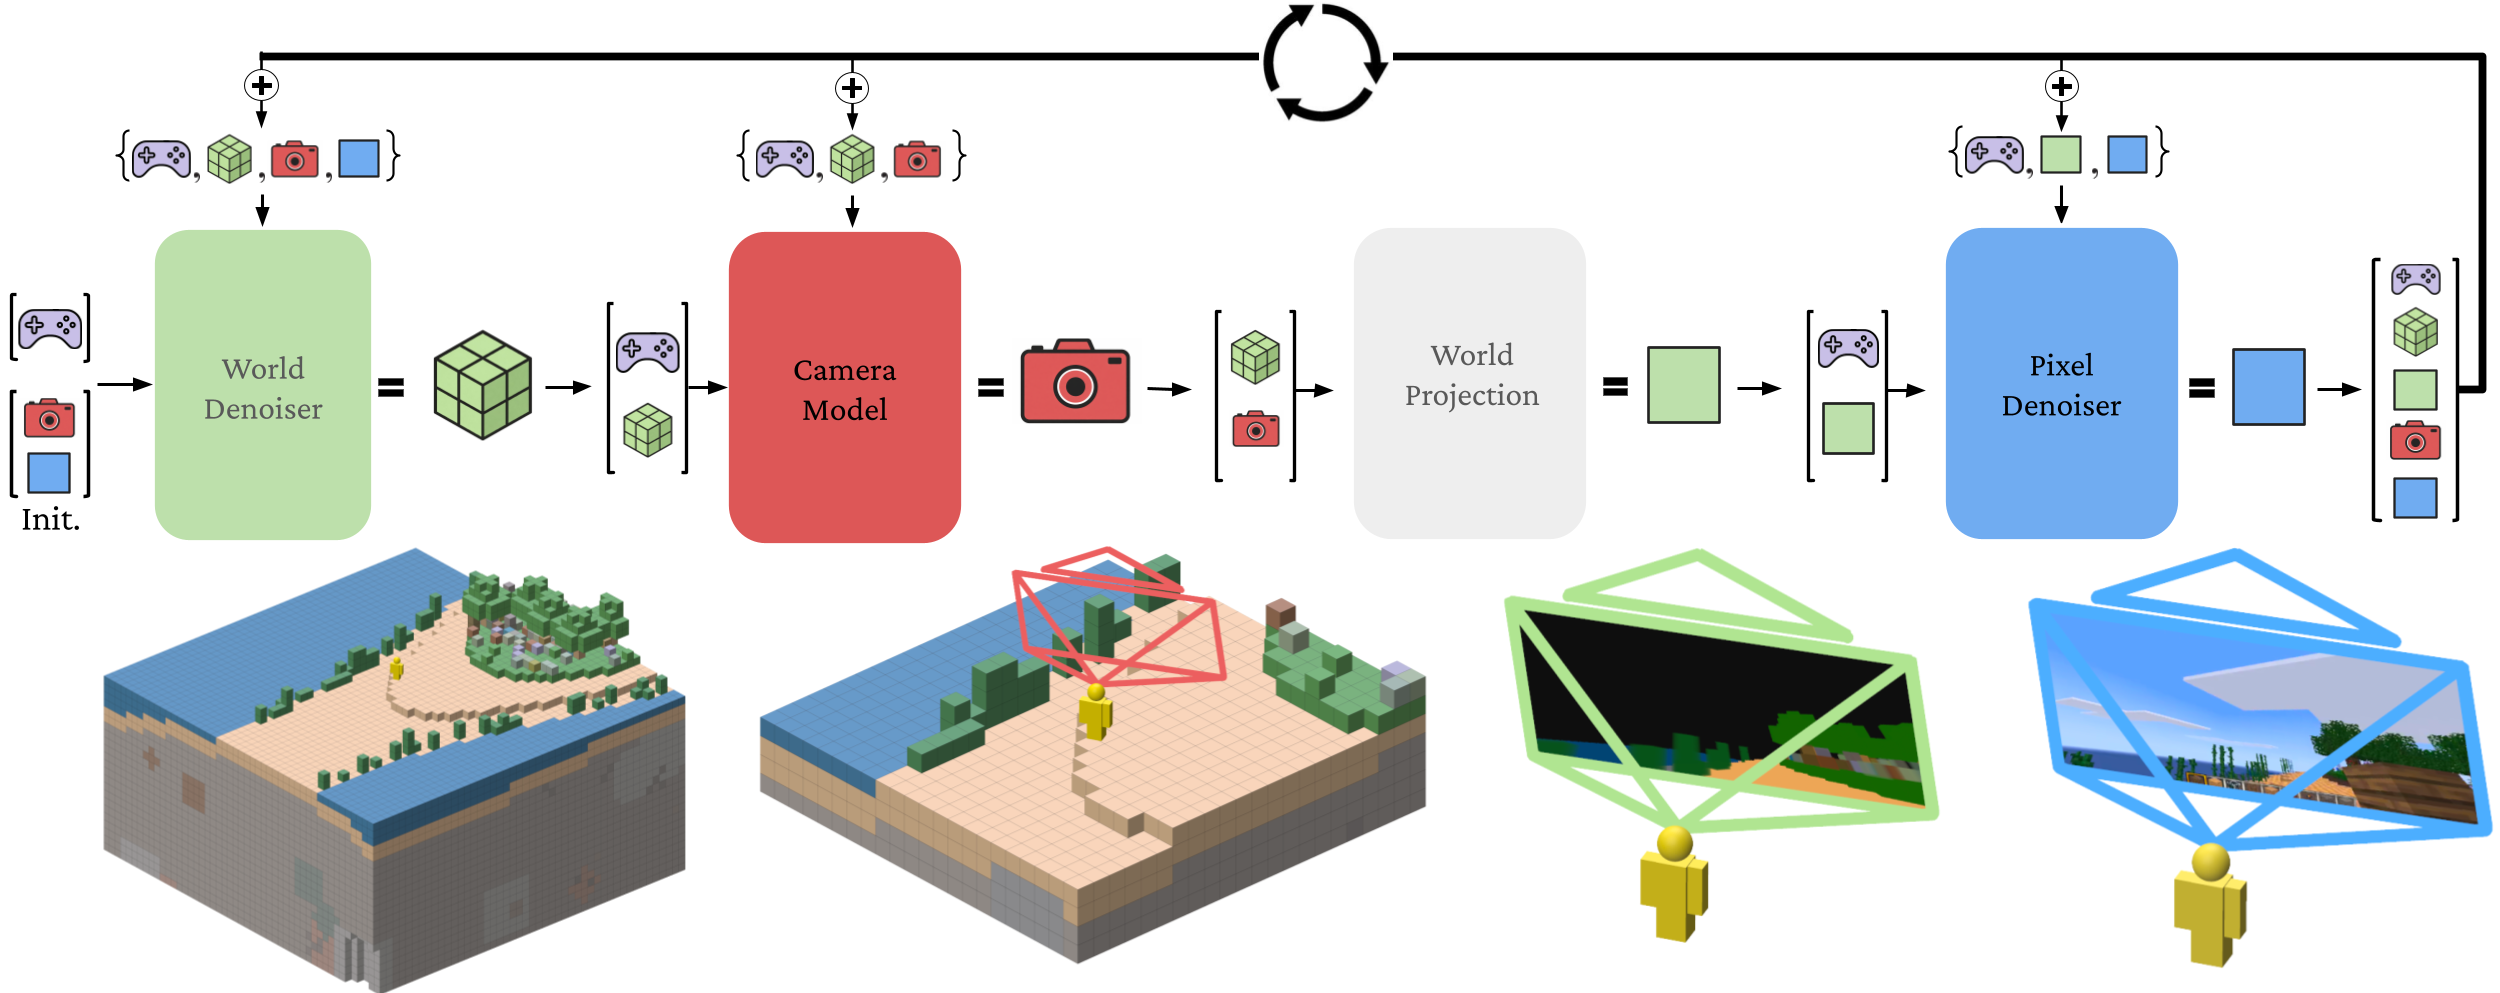
\includegraphics[width=\linewidth]{figs/Pipeline.png}}
    \caption{Initialized with a single-frame, PERSIST evolves in a four-part auto-regressive loop in response to user actions 
\includegraphics[height=1.5ex]{figs/action.png}. We first denoise the 3D environment centered on the agent in the form of a latent \textit{world-frame} 
\includegraphics[height=1.65ex]{figs/voxels.png}. Next, camera parameters 
\includegraphics[height=1.5ex]{figs/camera.png} are predicted with a feed-forward transformer. We then project the world to the camera plane to form a depth-ordered stack of world latents 
\includegraphics[height=1.5ex]{figs/voxel_frame.png}. Finally, pixel latents 
\includegraphics[height=1.5ex]{figs/pixel.png} are diffused, conditioned on pixel-aligned 3D information from the world frame.}
    \label{pipeline}
  \end{center}
\end{figure*}

\begin{figure*}[ht]
  \vskip 0.2in
  \begin{center}
    \centerline{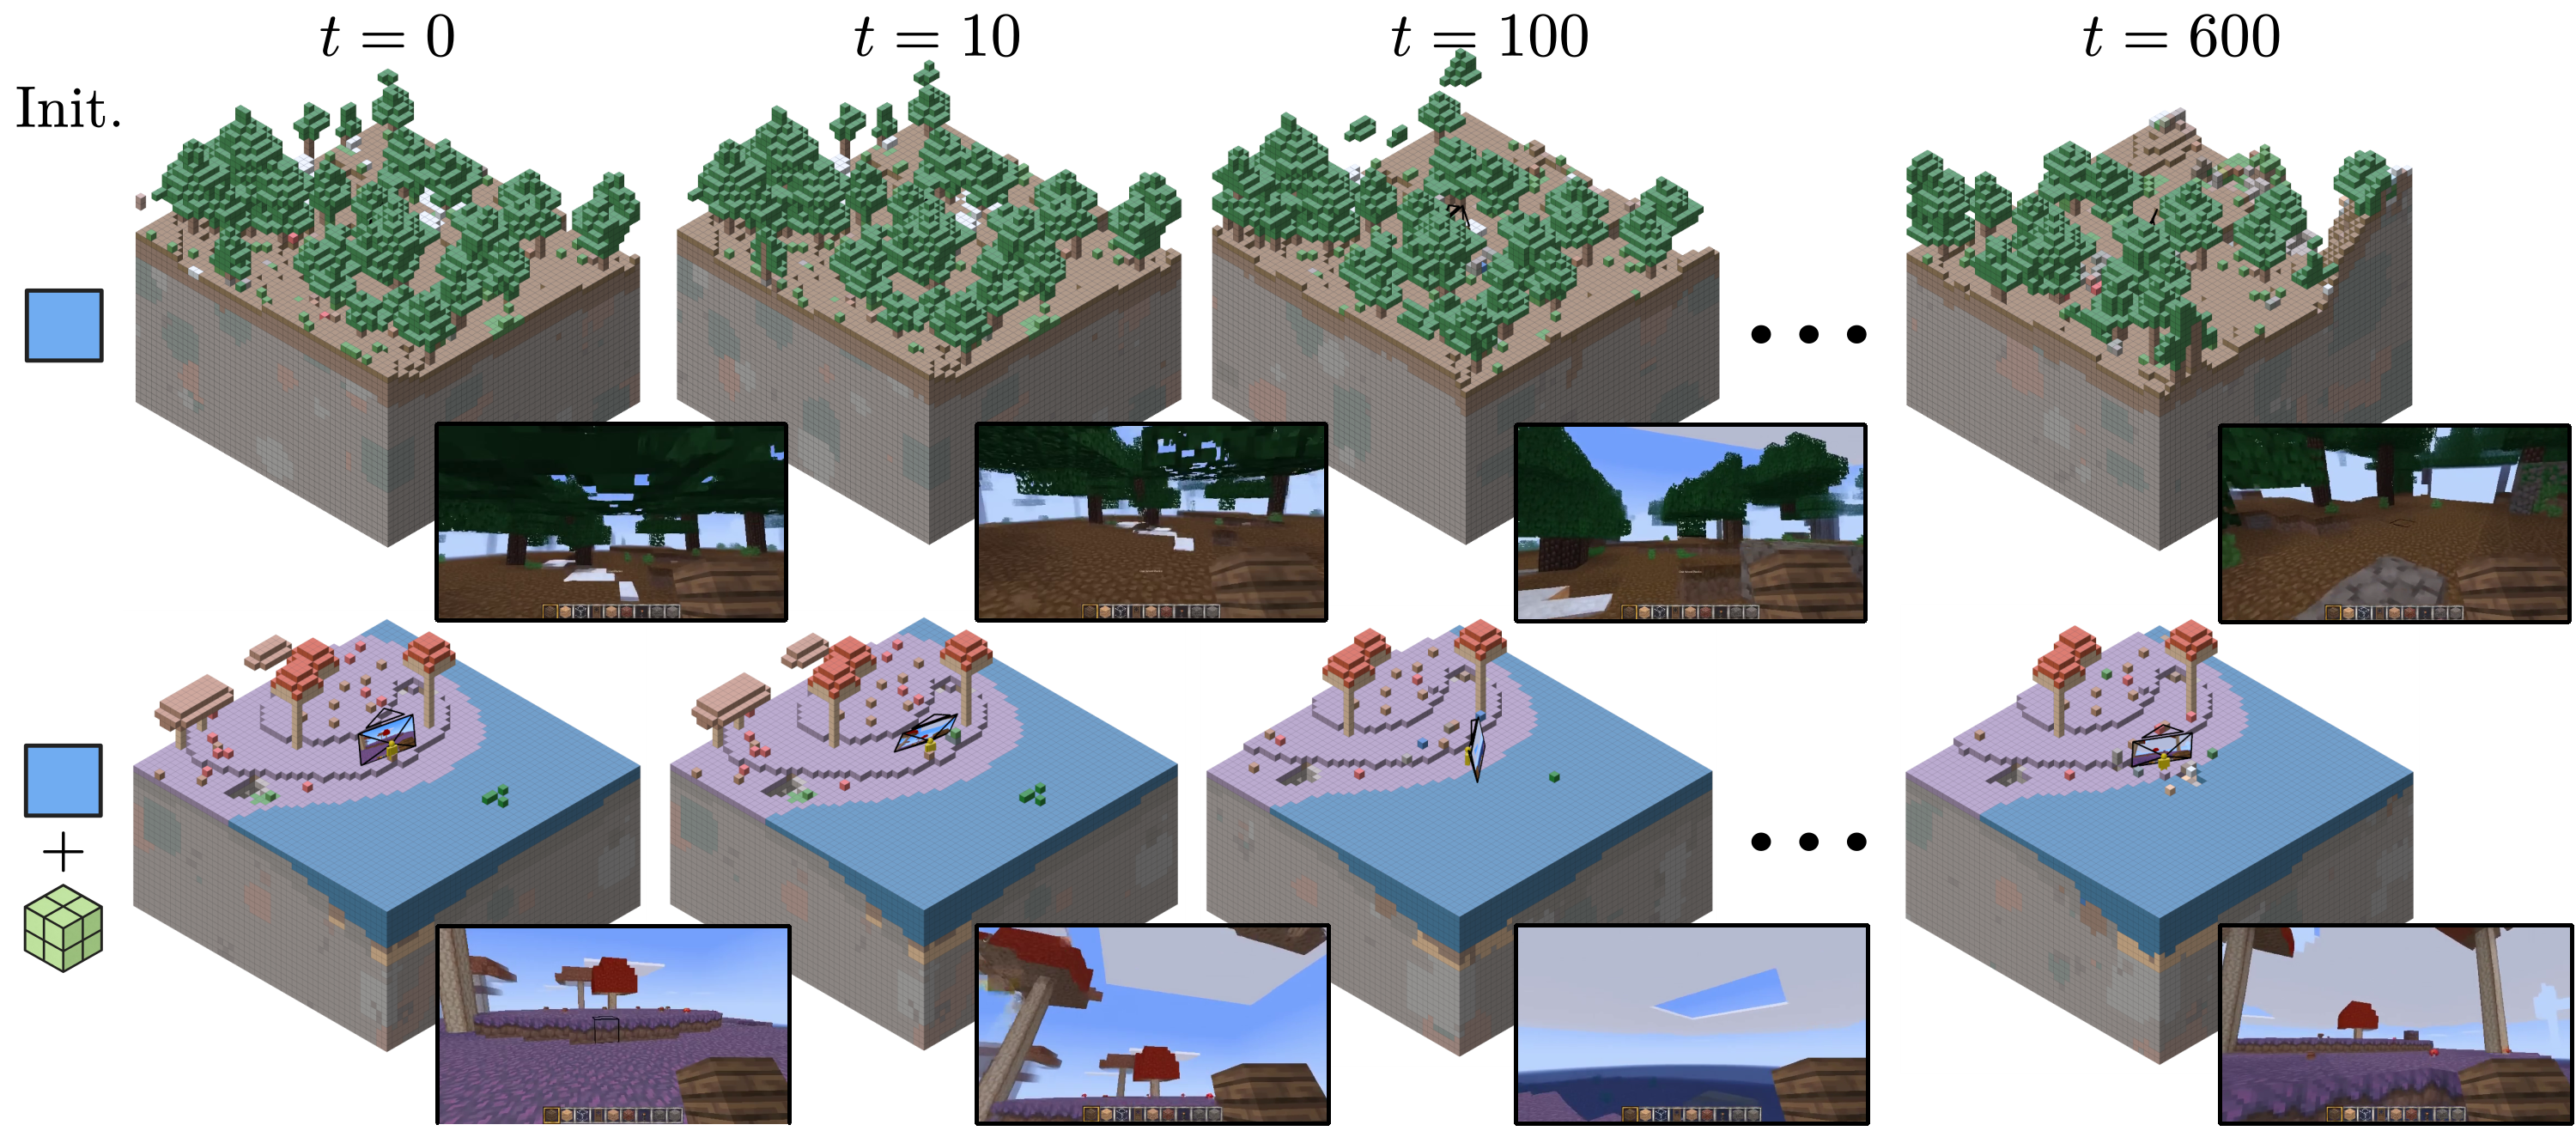
\includegraphics[width=\linewidth]{figs/qual.png}}
    \caption{Initalize with a single RGB frame, we visualize the world-frames and videos produced by an auto-regressive rollout of 600 timesteps.}
    \label{rollout}
  \end{center}
\end{figure*}


Interactive world models aim to generate experiences that unfold over time in response to user actions, enabling a new class of photo-realistic, personalised, and immersive interactive experiences for human users~\citep{kanervisto2025world, genie3, huang2025voyager}.
At the same time, such models hold significant potential for safely training embodied agents within simulators learned directly from data~\citep{hafner2025training,micheli2023transformers,alonso2024diffusion,garcin2024dred}.
Unlike passive video generation, interactive generation requires models to respond meaningfully to external interventions. In this setting, realism is not determined solely by per-frame visual quality, but by the degree to which the generated experience maintains persistent environments and stable dynamics throughout extended rollouts.

Most existing approaches to interactive video generation rely on auto-regressive (AR) models that condition on the history of past observations and actions to generate the most recent frame, often using diffusion- or flow-based transformers with causal attention~\cite{peebles2023scalable}.
This formulation is attractive: it naturally supports real-time action conditioning, allows generation to proceed indefinitely, and integrates cleanly with recent advances in large-scale video modelling.
As a result, AR video diffusion models form the backbone of many recent neural game engines and interactive world models~\citep{chegamegen,decart2024oasis,he2025matrix,xiao2025worldmem, valevskidiffusion,zhang2025matrix,yu2025gamefactory}.

However, conditioning on high-dimensional visual observations is computationally expensive, and the number of prior frames that AR models can ingest is tightly constrained by hardware.
In practice, this limits AR generation to condition on what amounts to only a few seconds of past footage, even when observations are compressed to lower spatial and/or temporal resolutions using learned autoencoders.
As a result, a growing body of work has explored how best to populate this limited contextual window, most commonly through heuristic strategies that retrieve individual key frames from a memory bank of past observations~\citep{xiao2025worldmem,huang2025memory}.

Yet, an inherent flaw of key-frame retrieval methods is that each pixel observation provides only partial, highly redundant, and viewpoint-dependent information about the world at a fixed point in time. As the memory bank grows, identifying the relevant past evidence becomes increasingly difficult.
As a result, generating extended coherent experiences within complex 3D environments remains an open challenge even for frontier models.\footnote{While not independently verifiable, closed-source models have reported achieving up to one minute of visual memory, representing the current claimed frontier of AR generation~\citep{genie3}.}

In this work, we propose to depart from pixel-based histories and substitute key frame retrieval with \textit{active key frame generation}.
We are inspired by traditional 3D simulators and game engines, which maintain coherence by directly rendering pixel frames from a persistent and dynamically evolving 3D state of the world.
We present PERSIST, a framework that brings persistence to learned AR world models.
PERSIST decomposes world simulation into three coupled components: a \textit{world-frame model} that predicts how an implicit, learned representation of a physical scene in three dimensions evolves over time, a \textit{camera model} that predicts the agent’s viewpoint within this scene, and a \textit{world-to-pixel generation module} that produces observations via differentiable projection and a learned rendering function.

Rather than treating pixels as the primary carrier of memory, PERSIST models both the structure and dynamics of the environment directly in latent 3D space.
This persistent world representation captures how the scene itself evolves over time, while the camera acts as a query mechanism that extracts the subset of 3D information relevant to guide the generation of the current frame.
This formulation enables long-horizon rollouts with fixed-cost memory, enforces geometric consistency by construction, and remains fully learned and compatible with modern diffusion- and flow-based training objectives.

We evaluate PERSIST in a large-scale voxel-based environment and find that explicitly modeling persistent 3D dynamics leads to substantially improved long-horizon generation quality compared to pixel-window and memory-retrieval baselines.
Our approach exhibits stronger temporal stability, improved spatial memory when revisiting previously observed regions, and markedly better 3D consistency overall.
Beyond quantitative gains, persistent world representation enables new capabilities, including explicit 3D scene initialization%, mid-episode scene edits, 
and the emergence of off-screen dynamic processes that continue to evolve even when not directly observed.

\section{Related Works}

%\paragraph{Rectified flow models.}
%Rectified flow treats generation as learning a velocity field that transports noise to data with low-variance supervision and efficient sampling~\citep{lipman2022flow}. This objective has been shown to be compatible with transformer backbones and latent-space training, and integrates with DiT-style architectures~\citep{peebles2023scalable}. Leveraging this compatibility, we parameterise both world-frame and pixel-space denoisers as conditional rectified flow models, thereby enabling action-conditioned denoising given a fixed context. This formulation supports efficient per-step updates that preserve training stability while reducing inference cost, while also keeping a single objective across modules and horizons.

\paragraph{Video denoising models.}
Recent advances in denoising models have led to substantial progress in video generation, extending image synthesis techniques to produce temporally coherent videos.
Recent methods adopt transformer-based designs, but are limited to denoising short clips due to the poor scaling of attention with video length. To address this, auto-regressive video generation has emerged as a promising direction for extending video sequences.
In this setting, rather than diffusing an entire sequence at a fixed noise level, frames are denoised sequentially, enabling potentially unbounded generation.

\paragraph{World models.} In parallel, world models aim to simulate environments by predicting future states conditioned on user actions, providing a foundation for model-based learning.
Advances in video generation have enabled high-fidelity interactive world simulation.
However, due to limited context windows, existing methods have to discard previously generated content, leading to temporal inconsistency and challenges with long-term spatial memory.
Recently, interactive world models have employed spatially-informed voting mechanisms to retrieve relevant frames.

\paragraph{3D Scene models}

% \todo[inline]{ <- May want a better title than that. Talk about models that generate a renderable 3D scene [e.g. Trellis, or its extension]. Sometimes it's explorable [e.g. Voyager, Worldlabs' paper etc]. But the scene is not interactive / dynamic. Instead we predict the dynamic 3D state of the world, modelling both dyamics processes (e.g. water flowing [if you want to give an example]) and player interacting with environment (e.g. player swimming, climbing [stop short of mentioning destroying / creating parts of the environment as we don't have conclusive proof for that capability yet.]) }

Unlike static 3D scene representations such as TRELLIS~\citep{xiang2024structured}, which focuses on generating high-fidelity geometry, our work focuses on the prediction of a dynamic 3D world state.
While recent advances in explorable environments such as World Labs~\citep{worldlab} or Voyager~\citep{huang2025voyager} allow for consistent navigation through a static scene, they often lack the capability to model complex and time-varying processes.
Our approach goes beyond passive observation by modeling both intrinsic environmental dynamics and agent-environment interactions.
By predicting the evolution of the underlying 3D state rather than just the visual surface, we enable a level of temporal and spatial consistency that reflects the active, changing nature of a truly interactive world.

\paragraph{Neural rendering.} In recent years, neural radiance fields have seen increasing usage in computer graphics as a compact and resolution-free parameterization of 3D scenes~\citep{mildenhall2021nerf, muller2022instant, li2023neuralangelo}.
Popularized by NeRF~\citep{mildenhall2021nerf}, these techniques rely on expensive ray-marching of an implicit function.
We take inspiration from a real-time graphics technique known as \textit{deferred shading}~\citep{deering1988triangle}: a mesh is first rasterized into a screen-space map of geometric information, which is then decoded pixel-wise into RGB values using a screen-space shader. 
Recently, learned neural deferred shaders~\citep{thies2019deferred, worchel2022multi, walker2023explicit} have proved to be efficient alternatives to ray-marching based neural renderers.
By leveraging highly-optimized polygon rasterization pipelines, they can achieve interactive frame rates across a wide range of compute platforms, including mobile devices~\citep{chen2023mobilenerf}.
However, these approaches have not seen much adoption due to their restriction to a fixed topology during training.
In this work, we assume a fixed topology in the form of grid mesh, on which geometric features can be efficiently rasterized. %\todo[inline]{WIP}

\section{Preliminaries}

\textbf{Rectified flow matching.} Our approach is based on the paradigm of flow matching and diffusion models~\citep{lipman2022flow}, where the task is to restore a clean data sample $x^0$ given a noised version $x^\tau$.
The noise level $\tau \in [0, 1]$ determines the degree of corruption of the data, where $\tau=0$ denotes clean data and $\tau=1$ indicates pure noise.
Rectified flow models~\citep{lipman2022flow,albergo2023building} employ a noising process $x^\tau = (1-\tau)x^0 + \tau x^1$ that linearly interpolates between sample $x^0$ and noise $x^1 \sim \mathcal{N}(0,\sI)$. 
Provided with a noised sample and corresponding noise level, the model $\gV_\theta$ is trained to predict the velocity vector $v = x^0 - x^1$ pointing towards the clean data via the conditional flow matching objective (CFM)~\citep{lipman2022flow}: 
\begin{equation}
    \mathcal{L}(\theta) = \norm{\gV_\theta (x^\tau, \tau) - (x^0 - x^1)}^2 \quad \tau \sim p(\tau),
\end{equation}
where $\tau$ is often sampled from a uniform or logit-normal distribution.
During inference, random noise $x^1$ is iteratively denoised into a clean sample $x^0$ over $K$ sampling steps, with uniform or variable step size $d^k$:
%
\begin{equation}
    x^{\tau - d^k} = x^\tau + \gV_\theta (x^\tau, \tau) d^k, \quad \tau \leftarrow \tau - d^k.
\end{equation}
\textbf{Autoregressive video generation.} While full-sequence video diffusion models treat videos as a single data sample to be denoised jointly at inference time, AR models treat videos as a sequence of individual frames $X^{n}_1 = x_1,x_2,\dots,x_n$ to be diffused sequentially.
\footnote{Notation-wise, the noise level of an individual frame $x^\tau_t$ is indicated by superscript $\tau$, its position in the sequence by subscript $t$.
In the case of a truncated sequence $X_k^{t}$, we overload the notation to have $k$ and $t$ indicate its beginning and end.} AR models employ causal masking strategies during training to ensure no information travels from the future into the past. Diffusion forcing~\citep{chen2024diffusion}
improves the generation stability of AR video diffusion models at inference by introducing per-frame noise levels that are sampled independently during training.
At inference, AR generation becomes a special case of the training setup, where the current frame is iteratively denoised from random noise and past frames receive a small fixed noise level $\tau_\text{ctx}$.

\textbf{Interactive world simulation.} Because generation proceeds step-by-step, AR models can in principle be unrolled indefinitely and conditioned on external control signals provided at each timestep.
This enables a transition from passive video generation to interactive world simulation. 

We employ a similar formalism as~\citet{valevski2024diffusionmodelsrealtimegame} to characterize the problem of learning a \textit{world model}, which we define here as a learned simulator of some \textit{interactive environment} $\mathcal{E}$.
$\mathcal{E}$ is specified by the tuple $\langle \mathbb{S}, \mathbb{O}, \mathbb{A}, \Omega, p\rangle$, where $\mathbb{S}$ is the space of latent states, $\mathbb{O}$ the space of observations, $\mathbb{A}$ the set of actions that may be taken within the environment, $\Omega : \mathbb{S} \rightarrow \mathbb{O}$ a partial projection function mapping states to actions and $p(s^\prime|a,s)$ is a transition probability function such that $s,s^\prime \in \mathbb{S}\times\mathbb{S}$ and $a \in \mathbb{A}$. 
Given a distribution of initial states and episode length $p_0$ and $N_0$, a policy $\pi$ in charge of selecting actions in $\mathcal{E}$ and a distance metric between observation sequences $D : \mathbb{O}^n \times \mathbb{O}^n \rightarrow \mathbb{R}$, learning an interactive world simulation of $\mathcal{E}$ consists of minimising the objective $\mathbb{E}[D(O^n, \tilde{O}^n)]$, where $O^n$ is a sequence of observations of length $n\sim N_0$ collected in $\mathcal{E}$ from starting state $s_0\sim p_0$ and by following $\pi$; and $\tilde{O}^n$ is obtained from an AR model $\gQ_\theta$ initialised at $\vo_0 = \Omega(s_0)$ and subjected to the same action sequence.

\section{A Persistent Environment Representation}
Learning $\gQ_\theta$ is often challenging when $\mathcal{E}$ is a complex 3D environment featuring high dimensional pixel observations.
First, memory constraints limit $\gQ_\theta$ to condition on a limited context window of past $K$ frames, imposing a constraint on temporal consistency once the generated episode exceeds $K$. 
Second, pixel observations generally provide partial information about the environment's hidden state, which can make learning transition dynamics challenging. %(for example when taking backwards steps while facing forwards). 
One solution would be to have $\gQ_\theta$ track the hidden state $s$. However, $s$ may be arbitrarily complex and/or not measurable --- in the case of a video game, $s$ represents the internal state of the game engine and its dynamic memory content.
Even if $s$ could be tracked, approximating $\Omega$ to recover the observation may be just as difficult.

Instead, we define a proxy $\tilde{s} = \langle \vw, \vc \rangle$, where $\vw$ is a \textit{world-frame} representing a fixed region of space centered on the agent, and $\vc$ encodes the agent's view within $\vw$.
Although not a perfect replacement for the hidden state, we argue that tracking $\tilde{s}$ is a highly effective modeling choice when $\mathcal{E}$ is a 3D environment, as it lets us:

\textbf{Simplify information retrieval.} At timestep $t$, $\vw_t$ takes on the role of \textit{spatial memory}, while $\vc_t$ acts as a lookup-key to extract spatial information from $\vw_t$ directly relevant to $\vo_t$.

\textbf{Improve dynamics predictions.} Tracking $\vw$ and $\vc$ simplifies modelling dynamics that would prove challenging under partial observability, such as interactions with out-of-view objects (e.g. modelling collisions), or tracking how occluded regions of the environment change over time.

\section{Methodology}
% \todo[inline]{Algo to describe sampling process of $\gQ_\theta$, complements figure 1 and describes different initialisation modes}
We present PERSIST (Persistent Environment Representations for Simulating Interactive Space-Time), a world simulation framework for complex 3D environments.
PERSIST decomposes the world simulation objective into the tasks of \textit{world frame prediction}, \textit{camera prediction} and \textit{world-to-pixel generation}.

\textbf{Data pre-processing.} The different components of PERSIST are trained from a dataset of trajectories collected from $\mathcal{E}$.
A trajectory consists of a sequence of pixel observations $O$, actions $A$, world-frames $W$ and camera views $C$.
In this work, we assume that $W$ and $C$ are directly obtainable from $\mathcal{E}$, the former as a 3D voxel grid encoding semantic information within a cuboid centered on the agent, and the later as a vector encoding the camera intrinsics and extrinsics.
Actions are embedded as a 23-dimensional multi-hot encoding of key presses and discretised mouse movements.
We train two separate VAEs (P-VAE and W-VAE) to encode base pixel- and world-frames into latent patches $\bar{\vo}$ and $\bar{\vw}$ of 10$\times$10 pixels and $4^3$ voxels respectively. 

\subsection{World-Frame and Camera Prediction}

\textbf{World frame prediction.} At each timestep, a new world-frame is generated by sampling 
\begin{equation}
  \bar{\vw}_t \sim \gW_\theta(\bar{\vw_t} | \bar{W}^{t-1}_{t-K}, A^t_{t-K}, C^{t-1}_{t-K-1}, \bar{O}^{t-1}_{t-K-1}),  
\end{equation}
where $K$ is the model's temporal context window and latents $\bar{W}^{t-1}_{t-K}$ and $\bar{O}^{t-1}_{t-K-1}$ are encoded using the VAEs. 
$\gW_\theta$ is parameterised as a rectified flow model with a causal Diffusion Transformer (DiT) backbone~\citep{peebles2023scalable} employing interleaved spatial, temporal and cross-attention modules.
We modify spatial modules to handle three spatial dimensions, and replace RoPE spatial embeddings~\citep{su2024roformer} with absolute position embeddings of the XYZ coordinates of the centroid of each voxel token.
We keep the temporal module as-is.
Actions and cameras are jointly embedded using a multi-layer perceptron (MLP).
The resulting embeddings are added to the denoising timestep embedding and injected into each module via Adaptive Layer Normalisation (AdaLN)~\citep{peebles2023scalable}.
We convey information on how individual pixel patches project to 3D space via Pl\"ucker embeddings~\citep{xiao2025worldmem,sitzmann2021light} which we compute from the cameras and concatenate to the channel dimension of the pixel patches.
The resulting patches are then injected via cross-attention.
Finally, we decode $\bar{\vw}_t$ back to its native resolution using the W-VAE.

Crucially, $\gW_\theta$ supports conditioning on $\bar{W}=\varnothing$, making it able of generating the initial world frame $\vw_0$ from initial condition $\langle \bar{\vo}_0, \vc_0 \rangle$ at inference time.
Thus, while we rely on $W$ to train $\gW_\theta$, we do not have to rely on ground truth 3D conditioning during inference.


% \textbf{Dynamic loss.}

\textbf{Camera model.} At any given timestep, cameras are represented as the 10-dimensional vector $\vc = [\textbf{pos}, \textbf{rot}, \text{fov}]$, where $\textbf{pos}\in \sR^3$ encodes the camera's position in the world-frame $\textbf{rot}\in \sR^6$ its orientation as a 6D continuous rotation~\citep{zhou2019continuity}, and $\text{fov}\in \sR$ its field-of-view. The camera model predicts $\vc_{t} = \gC_\theta (C^{t-1}_{t-1-K}, W^t_{t-K}, A^t_{t-K})$ using a 1D causal transformer backbone with RoPE temporal embeddings. Individual tokens are obtained by passing $\textbf{pos}$ and $\textbf{rot}$  through separate positional embedders, concatenating $\text{fov}$ and applying a linear projection. $W$ is cropped to its inner-most $4^3$ voxels and embedded alongside $A$ via a joint MLP prior to AdaLN injection. Given that the camera only rotates along its pitch and yaw axis, we re-parametrise the model's output layer to predict $\bar{\vc}=[\textbf{pos}, \Delta\textbf{rot}, \Delta\text{fov}]$, with residuals $\Delta\textbf{rot} = (\text{pitch}_t - \text{pitch}_{t-1},\text{yaw}_t - \text{yaw}_{t-1}) \in \sR^2$ and $\Delta \text{fov}=\text{fov}_t - \text{fov}_{t-1}$.\footnote{$\vc_t$ is recovered from $\langle \bar{\vc}_t, \vc_{t-1}\rangle$ via an algebraic manipulation at inference time.} The camera model is trained via MSE losses applied to $\textbf{pos}$, $\textbf{rot}$ and $\text{fov}$ with different coefficients.

\subsection{World-to-Pixel Generation}
In order to condition the pixel-space generation on 3D information we need to form world-to-pixel correspondence.

\textbf{World Projection.} %need to define what a rasteriser is either here or earlier in the text
Since we model a camera $\vc$ and 3D world-frame $\vw$, we can provide $\mathcal{P}_\theta$ with pixel-level conditioning on the relevant 3D features $\vw$ via a differentiable projection $\mathcal{R}(\vc, \vw)$ to screen-space. We then leave the final rendering step as a learned process for the screen-space denoiser $\mathcal{P}_\theta$. This choice allows the pixel denoiser to learn arbitrary compositing functions, whilst still enforcing geometric consistency through analytic projections of the 3D world.

\vspace{-0.35cm}
\begin{figure}[h]
    \centering
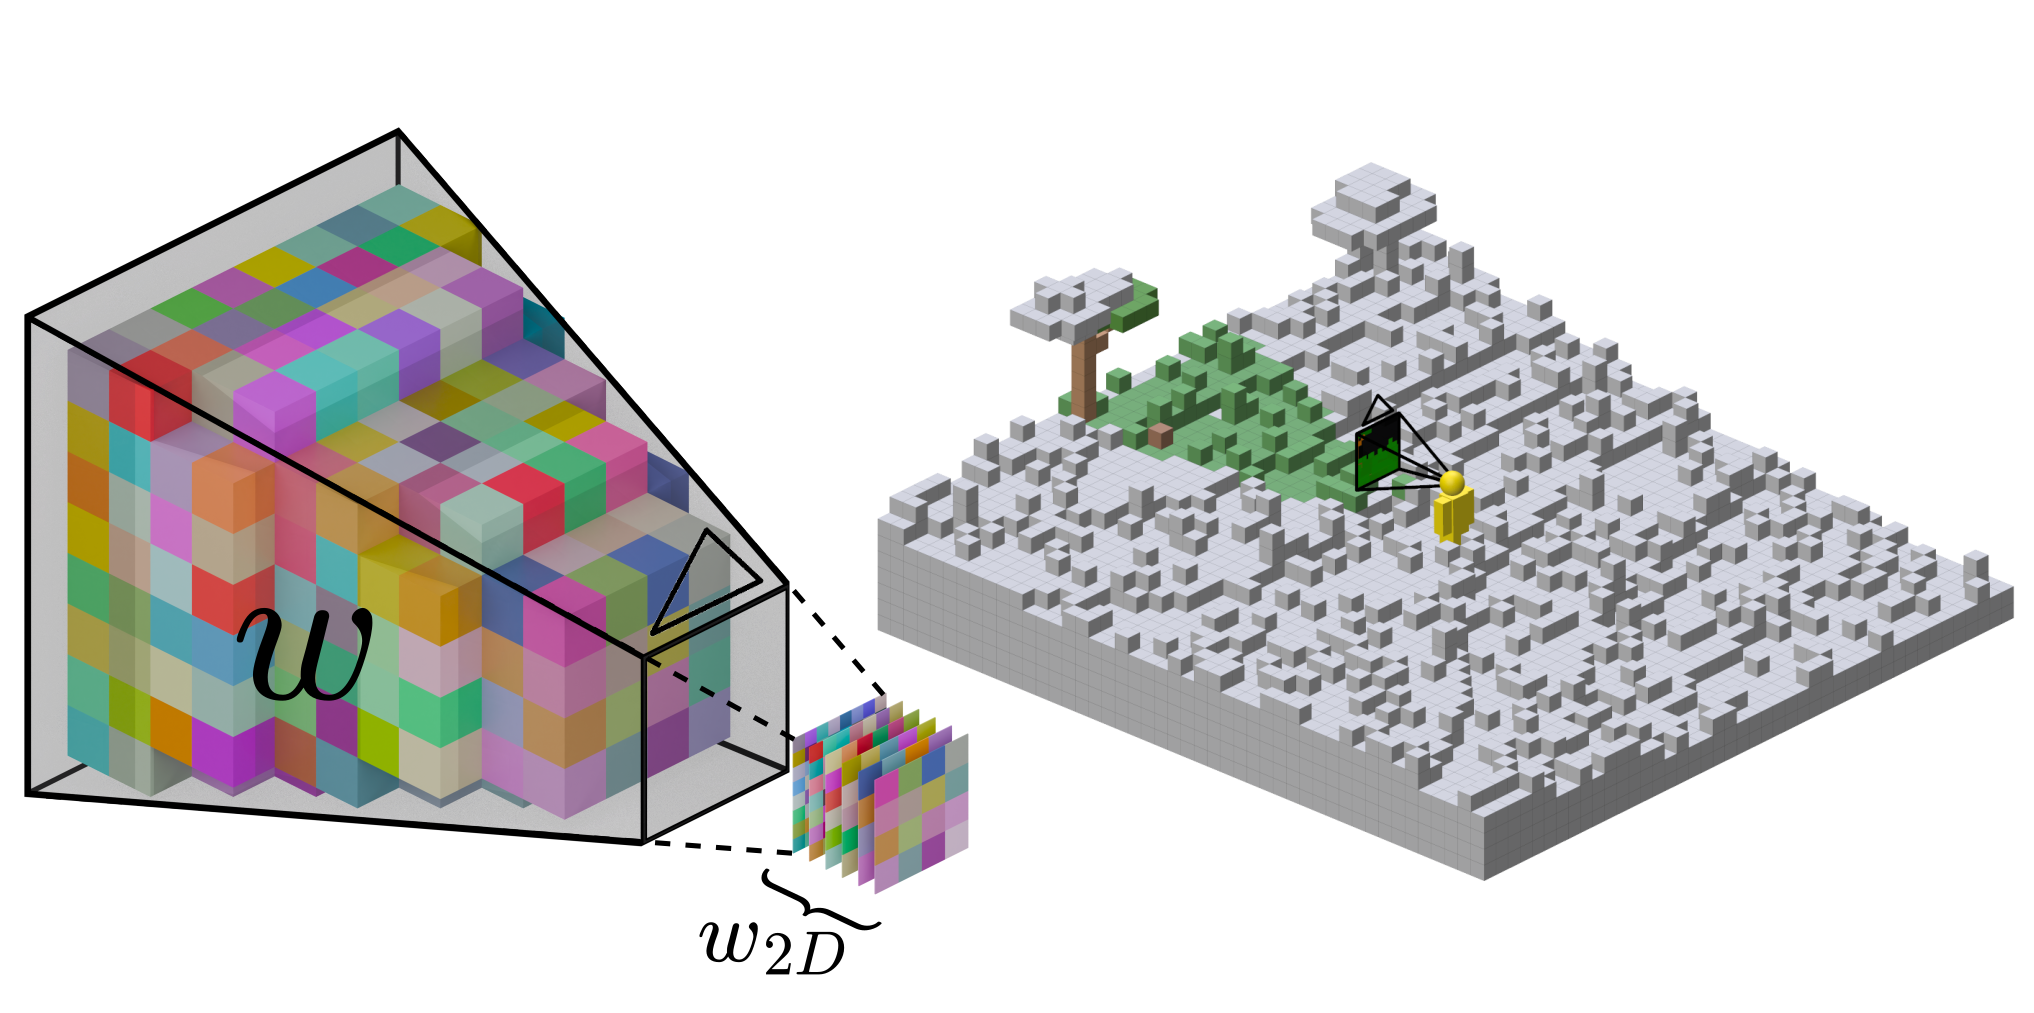
\includegraphics[width=1\linewidth]{figs/renderer_w.png}
    \caption{(Left) world frame $\vw$ features are projected to screen-space to form a depth-ordered stack of features $\vw_{2D}$. (Right) the world region fetched by the camera projection is displayed in colour.}
    \label{fig:placeholder}
\end{figure}

We define the projection operator $\mathcal{R}$ as 
\begin{equation}
    \mathcal{R}(\vc, \vw) = (\vw_{2D}, \vd), 
\end{equation}
where $\vw_{2D}  \in \mathbb{R}^{h \times w \times l \times m}$  represents a per-pixel depth-sorted list of $l$ voxel features with $m$ channels, and $\vd \in \mathbb{R}^{h \times w \times l}$ are their respective linear depths measured in camera space. To ensure pixel-level alignment between 2D and 3D latents, we rasterize $\vw$ using the same $h,w$ dimensions as the pixel latents. For projection, we use the CUDA-accelerated differentiable rasterization 
provided by~\citep{Laine2020diffrast}. For details, please see the appendix.
 

% For projecting, we leverage GPU-native triangle rasterization, by assigning voxel features to faces of a static voxel-grid mesh. Then, depth-peeling can applied during rasterization to produce a per-pixel, depth-ordered stack of 3D features $V_{2D}^{t} \in \mathbb{R}^{H \times W \times L \times C}$, where $L$ is the maximum number of layers. Since the mesh topology is fixed for a given resolution, we construct it once at initialization, updating vertex attributes ``on-the-fly" to avoid redundant mesh construction.  

While surrounding works~\cite{xiao2025worldmem,huang2025memory} use $\vc_t$ to retrieve a relevant key frame from a memory bank of past pixel observations, PERSIST employs $\mathcal{R}$ to \textit{generate} a key-frame from $\vw_t$ via a fixed-cost single feedforward operation.

\textbf{Screen space denoising.}
Finally, the pixel frame is obtained by sampling
\begin{equation}
    \bar{\vo}_t \sim \gP_\theta (\bar{\vo}_t | {W_{2D}}_{t-K}^{t}, A^t_{t-K}, \bar{O}^{t-1}_{t-K-1}).
\end{equation}
$\gP_\theta$ is parameterized as a rectified flow model with a casual DiT backbone employing interleaved spatial and temporal modules. Actions are embedded using a MLP and injected via AdaLN. Here, $\gP_\theta$ acts as a learned deferred shader, predicting information not provided by 3D latents (e.g. texture, lighting and particle effects, screen-space overlays).

Being directly projected in screen space, $\vw_{2D}$ provides pixel-aligned information and can be  directly incorporated to $\bar{\vo}$ via a channel-wise concatenation. We first append channel-wise the depth information $\vd$ to $\vw_{2D}$, and project the resulting vector to latent space via a 1D-convolution. Crucially, we assign more latent channels to $\vw_{2D}$ than to $\bar{\vo}$, in order to bias the model to use the 3D latent frame as its primary source of information.

\subsection{Mitigating Exposure Bias}

During training, the denoisers condition on latents encoded from the training data. However, at inference time, the 3D denoiser depends on latents predicted by the pixel denoiser, and vice-versa. To alleviate the resulting distributional shift caused by the denoisers' imperfect predictions, we apply a flat 10\% random noise augmentation to $\bar{O}$ when training $\gW_\theta$, and to $\bar{W}$ when training $\gP_\theta$. This lets us train each denoiser separately and combine them at inference time, without any fine-tuning being necessary.

\section{Experiments}

\begin{figure*}[ht]
  \vskip 0.2in
  \begin{center}
    \centerline{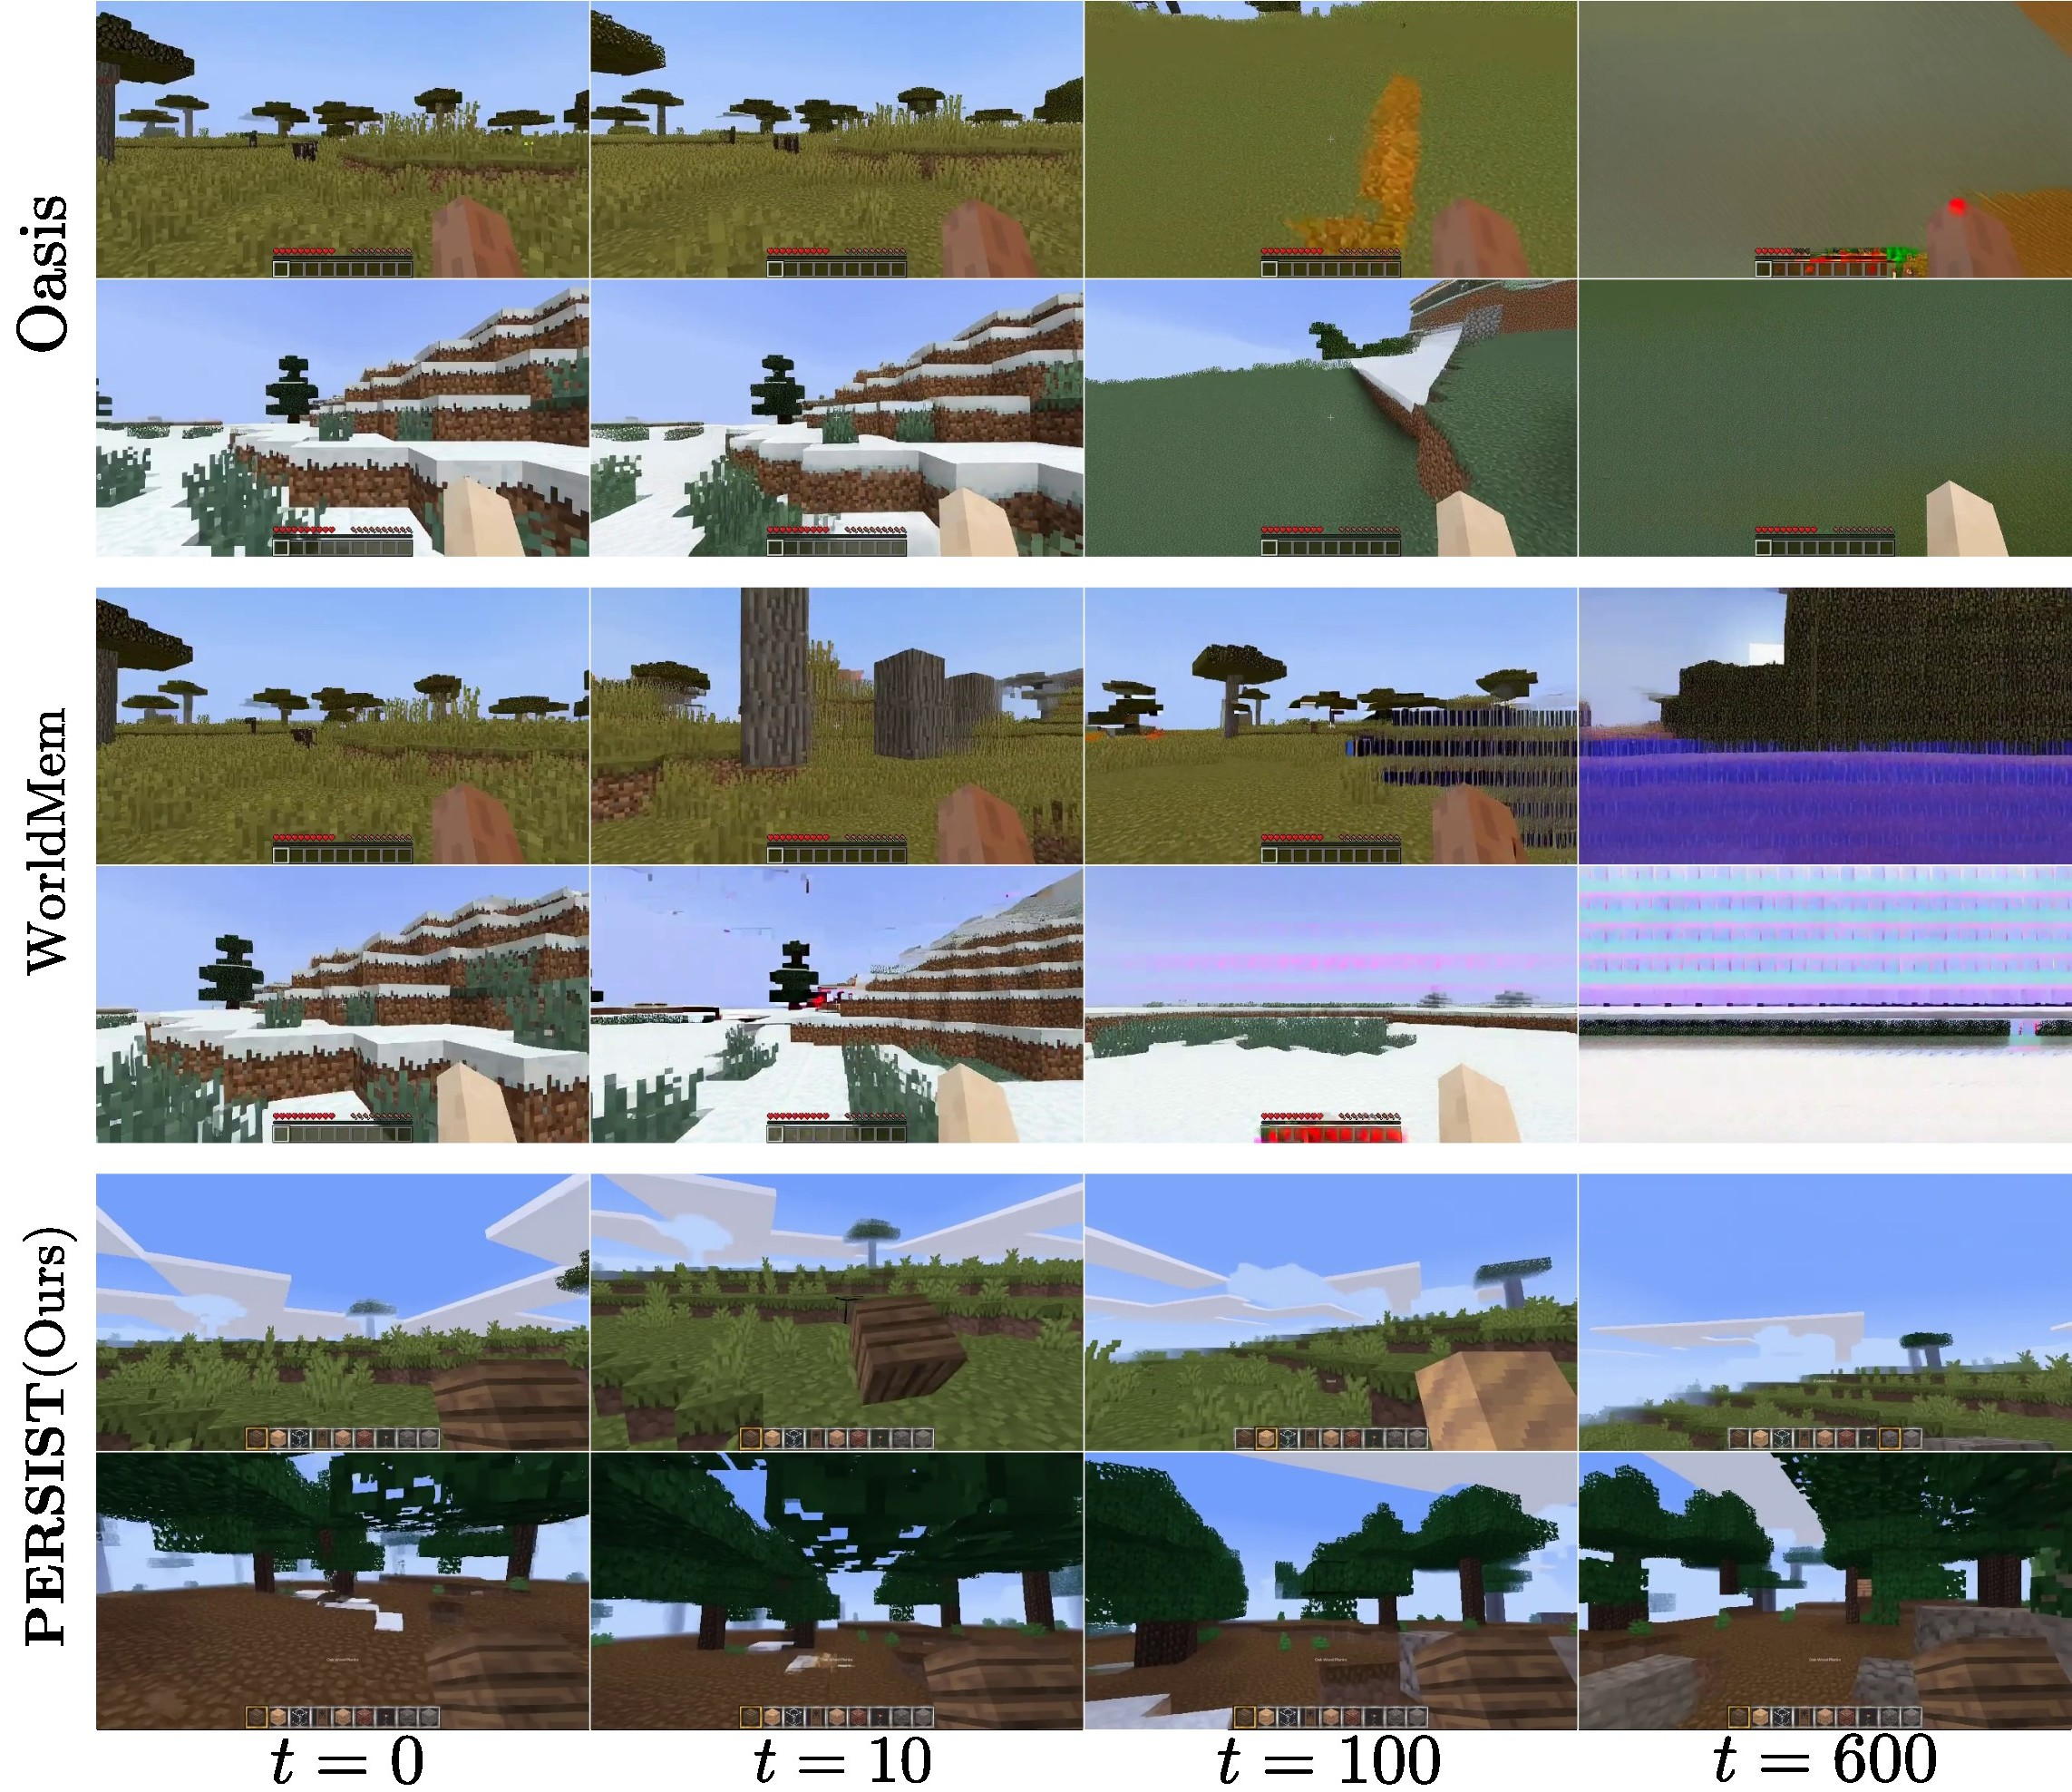
\includegraphics[width=\linewidth]{figs/compare.jpg}}
    \caption{Qualitative Comparison between PERSIST (Ours), Oasis~\citep{decart2024oasis} and WorldMem~\citep{xiao2025worldmem}.}
    \label{rollout}
  \end{center}
\end{figure*}

We conduct our experiments within Luanti~\citep{luanti2024}, an open-source voxel-based game engine inspired by Minecraft. Voxel environments constitute a valuable research platform~\citep{malagon2025craftium,fan2022minedojo,guss2019minerl,baker2022video}, as they instantiate complex, diverse, and persistent 3D worlds with rich player–environment interactions. Unlike prior work that learns world models from data collected within a single fixed game map~\citep{alonso2024diffusion,kanervisto2025world},we instead consider learning from a broad distribution of procedurally generated worlds. This setting substantially increases the difficulty of achieving spatial and temporal consistency, as models cannot rely on overfitting to a single underlying layout.

We select Luanti due to its open-source design and expressive Lua API, which facilitates data collection. In Luanti, the world-frame $\vw$ is represented as a 3D grid of semantic voxel values centered on the agent. This representation is easily interpretable, facilitating controlled experimentation while significantly accelerating research and analysis.

\textbf{Dataset.} We use the Craftium platform~\citep{malagon2025craftium} to collect data to train and evaluate our models. We collect approximately 100K trajectories, amounting to roughly 40M individual environment interactions or 460 hours of gameplay recorded at 24Hz.
To interact with the game, we employ a similar strategy as~\citep{yu2025gamefactory} and design a simple policy that randomly samples from a set of pre-defined action sequences. \Cref{app:data} provides further details regarding our data collection strategy.

\textbf{Training and Inference.} All models are trained using the AdamW~\citep{loshchilov2018decoupled} optimizer with a learning rate of $1e-4$. We first train the VAEs and pre-encode the 3D and pixel latents to accelerate the training of the dynamic models. The pixel and 3D VAEs take 4 and 12 days to train using 8 A100 GPUs. We train two versions of the 3D denoiser, ``3D-Small'' and ``3D-XL'', which uses 8$\times$ more spatial tokens. 3D-Small takes 3 days to train on 8 H100 GPUs, while 3D-XL and the pixel denoiser each take 10 days. The camera model trains on a single A100 in 16 hours with batch size 256. All other models use batch size 64. Each model is trained separately and assembled in the full pipeline with no further finetuning. At inference, we use 20 denoising steps per-frame and sligtly noise past generated frames to make the denoisers more resilient to imperfections in their own generations. We provide more implementation details in \Cref{app:model}.

\begin{table*}[t]
  \centering
  \caption{Comparison across evaluation modes.}
    %\rowcolors{2}{gray!8}{white}
    \begin{tabular}{lccccc}
    \toprule
    Method & FVD & Visual Fidelity & 3D Consistency & Temporal Consistency & Overall Score \\
    \midrule
    PERSIST-Base & 209 & 2.5 $\pm$ 0.18 & 2.6 $\pm$ 0.19 & 2.6 $\pm$ 0.2 & 2.6 $\pm$ 0.18 \\
    PERSIST-XL & 181 & \textbf{2.8 $\pm$ 0.16} & \textbf{2.8 $\pm$ 0.15} & \textbf{2.9 $\pm$ 0.16} & \textbf{2.9 $\pm$ 0.15} \\
    PERSIST-XL$+\vw_0$ & \textbf{116} & \textbf{2.9 $\pm$ 0.18} & \textbf{2.7 $\pm$ 0.23} & \textbf{2.7 $\pm$ 0.26} & \textbf{2.8 $\pm$ 0.22} \\
    Oasis & 706 &2.2 $\pm$ 0.15 & 2.0 $\pm$ 0.16 & 1.9 $\pm$ 0.16 & 2.0 $\pm$ 0.15 \\
    WorldMem & 596 &1.7 $\pm$ 0.12 & 2.0 $\pm$ 0.15 & 1.8 $\pm$ 0.15 & 1.8 $\pm$ 0.13 \\
    \bottomrule
    \end{tabular}
  \label{tab:eval}
\end{table*}



\subsection{Interactive Generation}

In this section, we assess our method's ability to generate interactive experiences that are both spatially and temporally consistent. We craft action policies specifically designed to make the agent explore its environment while continually revisiting previously rendered locations at different times and from various viewpoints.
%  \todo[inline]{Mention trajectory lengths? very long rollouts? Define trajectory archetypes here or in the results table?}
 We deploy these policies in Craftium to collect a dataset of 148 evaluation trajectories from game worlds that were held-out from the training set. Finally, we sample starting conditions $\langle \vo_0, \vc_0\rangle$ and action sequence $A$ from the evaluation set to generate trajectories with PERSIST-S (featuring the 3D-Small denoiser) and PERSIST-XL (featuring the 3D-XL denoiser).

% old baseline section with more baselines, to add back for rebuttals
% \textbf{Baselines.} We compare our approach against Oasis [ref] and MineWorld [ref], two approaches conditioning directly on a past pixel observation window, as well as WorldMem [ref] and MemoryForcing [ref] which incorporate key-frame retrieval from a memory bank of past pixel observations. As these methods were trained with Minecraft data, we collect a separate evaluation set in Minedojo [ref] using the same evaluation policies, in order to not induce any domain shift and we replicate the baselines' respective inference configurations. In the case of WorldMem and MemoryForcing, this includes initialising their memory bank with 200 ground truth cameras and pixel observations, and providing ground truth cameras alongside actions during inference.

\textbf{Baselines.} We compare our approach with Oasis~\citep{decart2024oasis} and WorldMem~\citep{xiao2025worldmemlongtermconsistentworld},  two interactive video generation methods employing the same DiT backbone as $\gP_\theta$, but directly conditioning generation on observations from $O^{t-1}$.
Oasis conditions on the most recent $O^{t-1}_{t-K}$ observations, and can therefore also be viewed as an ablation of PERSIST in which the guidance provided by $W_{2D}$ is disabled.
WorldMem actively tracks cameras during generation, and retrieves frames from $O^{t-1}$ closely matching its current camera prediction to use as key-frames to guide generation.
As these methods were trained using Minecraft data, we collect a separate evaluation set in Minedojo~\citep{fan2022minedojo} to not induce domain shift, and we replicate their respective inference configurations.
In the case of WorldMem, this includes initialising the memory bank used to sample key-frames with 600 ground truth cameras and pixel observations.
This contrasts with PERSIST, which is initialised from a single initial frame $\langle \vo_0, \vc_0 \rangle$.

% \textbf{Qualitative analysis.} \todo[inline]{write once we get to look at rollouts. Highlight problems with baselines etc}

% placeholder for results:
% FVD oasis: 705.6
% FVD world mem: 595.7 
% FVD PERSIST-Small
% FVD PERSIST-XL
% FVD PERSIST-XL + W_0

% For appendix
% Self-FVD Minetest: 62.5
% Self-FVD Minedojo 44.7

\textbf{User study.} In addition, we conduct a user study consisting of 300 evaluation trials, in which users are asked to score videos on their ``Per-Frame Visual Fidelity'', their ``3D Spatial Consistency'', and their ``Temporal Environment Stability and Consistency'' before assigning an overall score. We complement this study with computing the Frechet Video Distance (FVD)~\citep{unterthiner2018towards} between each method and its respective evaluation set. Supplementing the FVD with a user evaluation is of particular interest to us, as the FVD measures the distance between the generated and ground truth videos, but does not directly assess spatial and temporal consistency for individual episodes. %Each trial consists of a pair of videos sampled at random from a pool consisting of generations obtained from our approach, the baselines and both evaluation sets. \todo[inline]{describe results. Maybe a good way to remotivate FVD measurements if Overall Scores and/or Visual quality and 3D consistency scores align with quantitative rankings}

\textbf{Quantitative analysis.} We report results in \Cref{tab:eval}. Across all evaluated metrics, each PERSIST configuration significantly outperforms all baselines, demonstrating the robustness of our framework. Improvements are consistent across both spatial and temporal consistency metrics, indicating that explicitly modelling a persistent 3D environment state yields systematic gains rather than isolated metric-specific effects. Among user-study metrics, the smallest performance gap with prior work occurs for per-frame visual quality when compared against Oasis. This result aligns with our design intent: PERSIST primarily targets long-horizon spatial and temporal consistency rather than frame-level appearance. Nonetheless, improvements in reported visual fidelity are significant, suggesting that PERSIST reduces the occurrence of visual artifacts. Finally, PERSIST-XL variants are scored consistently higher than the PERSIST-Base configuration across all metrics, confirming that scaling the number of 3D spatial tokens of $\gW_\theta$ translates directly into improved world modelling performance.

% Notes on eval set:
% - describe eval set, make distinction between two type of trajectories: 
%        - Orbit: specifically designed to challenge spatial +  temporal consistency (spatial: viewing object/scenes from different view points, temporal: revisiting already explored locations/views)
%        - Free-Play: Agent perform randomised actions in the environment
%        - Exploration: Actions are aimed to cover a large distance (more timesteps, agent moves forward/backward and spins on itself periodically)


% Notes on Baselines:
% - describe baselines and highlight inherent limitations: e.g. Oasis/Mineworld have no memory mechanism (but Oasis uses 2x temporal context window as our models). WorldMem/MemoryForcing require hundred of GT frame to be warm-started at inference.
% - mention a separate eval set is collected in MineDojo to not induce domain shift for baselines.
% - mention our training set if much smaller than VPT training set (check size but I think 10-100x smaller

\subsection{New Applications and Emerging Capabilities}

In addition to maintaining strong spatial and temporal consistency over experiences spanning hundreds of frames, we discover additional capabilities afforded by our 3D dynamic model.

%Todo: example
\textbf{Explicit 3D initialisation.} At the start of an episode, we may directly provide a custom $\vw_0$ to the generation pipeline, instead of having it generated by $\gW_\theta$. This explicit conditioning provides a greater degree of control over the generated experience than providing an image, as the full surroundings of the agent are directly specified. We observe a marked improvement in FVD when comparing PERSIST-XL+$\vw_0$ with PERSIST-XL (\Cref{tab:eval}), indicating PERSIST-XL+$\vw_0$ is successfully conditioning and maintaining the ground-truth 3D information about the environment. Crucially, PERSIST-XL+$\vw_0$ and PERSIST-XL perform similarly in user-ratings, which strongly indicates that PERSIST-XL is capable of generating plausible and self-consistent environments without requiring 3D ground truth information at initialisation.

% \textbf{World edits mid-generation.} [ref GameNGen, WHAM] proposed to perform manual edits to the generated pixel frames before re-injecting them as context, as an alternative way of influencing the generated experience. Similarly, as we can extract $\vw_t$ at any point during generation, we obtain the capability of making precise 3D-edits to the world mid-episode. To do so, we pause generation after timestep $t$ and manually edit $\vw_t$ to obtain $\tilde{\vw}_t$. We then restart generation using $\{\tilde{\vw}_t, \vc_t, \vo_t, \va_t\}$ as the starting condition. We show a few examples of this in \Cref{fig:world-edits}.

% \textbf{Persistent world dynamics.} In \Cref{fig:waterfall}\todo{fig}, we show how PERSIST learns to model dynamic processes in the environment, such as a water falling on top of the player. Such environment dynamics remain actively modeled even while they are not rendered to screen space: a few seconds later, as the player revisits its prior location, the waterfall is present and is slowly flooding the area.

\section{Conclusion}

In this work, we introduced PERSIST, a world modeling framework that moves beyond pixel-based histories by explicitly modeling the evolution of a persistent latent 3D state. Our results demonstrate that actively generating guidance frames from this 3D state substantially improves spatial memory, temporal coherence, and overall generation quality compared to AR approaches conditioning on a limited window of past pixel observations, or retrieving key frames from a memory bank. In addition, we show that explicitly tracking the 3D state of the world leads to novel ways of controlling generated experiences, by allowing to pre-specify, visualise and modify the structure of generated environments.

\paragraph{Current limitations.} While PERSIST yields substantial improvements in generation quality, temporal stability, and environmental coherence, human evaluators consistently assign higher scores to ground-truth videos, with average ratings in the range of 4.0–4.3 across metrics and a lower variance. This gap highlights that accurately and robustly modelling complex 3D environments over extended interactions remains an open challenge. In our generated rollouts, we observe gradual degradation in visual quality and physical stability over time, occasionally manifesting as artifacts such as minor jittering or imperfect player–environment alignment (e.g., floating effects). We attribute these behaviours primarily to exposure bias: during inference, each component of the pipeline must condition on its own predictions as well as those of other models, despite having been trained independently using ground-truth targets. This mismatch leads to compounding errors and imperfect dynamics, although PERSIST remains substantially more stable than all evaluated baselines. We expect that incorporating an additional fine-tuning stage in which the full pipeline is trained on its own autoregressive rollouts would further improve long-horizon stability, as demonstrated in recent work~\citep{huang2025self}. We leave an investigation of this direction to future work.

\paragraph{Future work.} PERSIST currently assumes access to ground-truth 3D information and camera poses during training, which restricts its applicability to settings where such information can be obtained, for instance from game engines, simulators, or datasets containing 3D annotations~\citep{zhou2018stereo,Matterport3D,yeshwanth2023scannet++}.
An important direction for future work is to relax this requirement by leveraging recent advances in 2D-to-3D foundation models~\citep{wang2025vggt,sam3dteam2025sam3d3dfyimages} to estimate world structure and camera parameters directly from pixel observations as a pre-processing step.
PERSIST presently tracks a fixed region of 3D space centered on the agent, causing information outside this region to be discarded as the agent moves through the environment.
Enabling dynamic loading and unloading of spatial chunks from a 3D memory bank would provide a natural path toward scaling PERSIST to retain spatial information over arbitrarily large environments.
Finally, extending PERSIST to model multiple agents within a shared world-frame represents an exciting avenue for future work, opening the door to multi-agent interaction within coherent, persistent environments.

\section*{Impact Statement}

This work advances the field of Machine Learning by improving the spatial and temporal consistency of generative world models.
While our research is primarily conducted within the simulated environment of Luanti, the underlying methodologies have potential applications in video games, digital twin simulation, and embodied AI navigation, where reliable 3D scene representation is critical.
We do not foresee any immediate negative societal consequences that require specific highlighting at this stage, as our model operates within a synthetic domain.

% In the unusual situation where you want a paper to appear in the
% references without citing it in the main text, use \nocite
% \nocite{langley00}

\bibliography{biblio}  
\bibliographystyle{icml2026}

%%%%%%%%%%%%%%%%%%%%%%%%%%%%%%%%%%%%%%%%%%%%%%%%%%%%%%%%%%%%%%%%%%%%%%%%%%%%%%%
%%%%%%%%%%%%%%%%%%%%%%%%%%%%%%%%%%%%%%%%%%%%%%%%%%%%%%%%%%%%%%%%%%%%%%%%%%%%%%%
% APPENDIX
%%%%%%%%%%%%%%%%%%%%%%%%%%%%%%%%%%%%%%%%%%%%%%%%%%%%%%%%%%%%%%%%%%%%%%%%%%%%%%%
%%%%%%%%%%%%%%%%%%%%%%%%%%%%%%%%%%%%%%%%%%%%%%%%%%%%%%%%%%%%%%%%%%%%%%%%%%%%%%%
\newpage
\appendix
\onecolumn
\section{Model hyperparameters.}\label{app:model}

\begin{table}[htb!]
\centering
\begin{tabular}{cc}\toprule  
Parameter & Value \\
\midrule
input shape & [48, 48, 48, 2415] \\
number of residual blocks & 2 \\
middle channels & [32, 128, 512] \\
latent channels & 48 \\
\bottomrule
\end{tabular}\caption{W-VAE configurations.}
\label{table:w-vae}
\end{table}

\begin{table}[htb!]
\centering
\begin{tabular}{cc}\toprule  
Parameter & Value \\
\midrule
input size & [360, 640, 3] \\
patch size & 10 \\
latent dimension & 16 \\
encoder dimension & 1024 \\
encoder depth & 6 \\
encoder number of heads & 6 \\
decoder dimension & 1024 \\
decoder depth & 12 \\
decoder number of heads & 16 \\
\bottomrule
\end{tabular}\caption{P-VAE configurations.}
\label{table:p-vae}
\end{table}

\begin{table}[htb!]
\centering
\begin{tabular}{cc}\toprule  
Parameter & Value \\
\midrule
voxel shape & [48, 16, 16, 16] \\
hidden dimension & 128 \\
latent dimension & 64 \\
pixel shape & [16, 64, 36] \\
hidden dimension & 64 \\
latent dimension & 32 \\
fusion hidden dimension & 512 \\
output dimension & 8 \\
context window size & 8 \\
camera context hidden dimension & 256 \\
camera context number of heads & 8 \\
camera context number of layers & 3 \\
action dimension & 23 \\
action context hidden dimension & 256 \\
action context number of heads & 8 \\
action context number of layers & 3 \\
\bottomrule
\end{tabular}\caption{Camera model configurations.}
\label{table:cam-model}
\end{table}

\begin{table}[htb!]
\centering
\begin{tabular}{cc}\toprule  
Parameter & Value \\
\midrule
input shape & [16, 16, 16, 48] \\
patch size & 2 \\
hidden size & 1024 \\
depth & 12 \\
number of heads & 16 \\
mlp ratio & 4.0 \\
pixel condition shape & (16, 36, 64) \\
pixel condition patch size & 2 \\
cross condition hidden size & 1024 \\
action condition dimension & 23 \\
camera condition dimension & 8 \\
context window size & 8 \\
\bottomrule
\end{tabular}\caption{World denoiser configurations.}
\label{table:world-denoiser}
\end{table}

\begin{table}[htb!]
\centering
\begin{tabular}{cc}\toprule  
Parameter & Value \\
\midrule
input shape & [16, 32, 16] \\
patch size & 2 \\
hidden size & 1024 \\
depth & 12 \\
number of heads & 16 \\
voxel dimension & 48 \\
\bottomrule
\end{tabular}\caption{Pixel denoiser configurations.}
\label{table:pixel-denoiser}
\end{table}

\clearpage
\section{Evaluation Data and User Study}\label{app:data}

As discussed in the main body, we curated evaluation datasets across four modes to assess agent behavior: \textit{Free Play}, \textit{Move Forward}, \textit{Move Backward}, and \textit{Orbit}.
These modes are designed to highlight explorative behaviors that demand high levels of temporal and spatial consistency.

\begin{itemize}
    \item \textbf{Free Play:} The agent follows a predefined stochastic sampling rule to execute random actions, facilitating diverse environmental exploration.
    \item \textbf{Move Forward/Backward:} The agent performs a directed linear translation (forward or backward) followed by a rotational ``look around'' maneuver to observe the surroundings.
    \item \textbf{Orbit:} The agent adheres to a policy that maintains a constant radius while rotating around a fixed central coordinate.
\end{itemize}

For inference with \textit{WorldMem}, we prepend 600 context frames, collected within \textit{MineDojo}, to the evaluation sequence to provide necessary historical state information.

\subsection{User Study Protocol}
The user study was deployed via a custom web interface (see Figure~\ref{fig:ui_screenshot}). Participants were tasked with performing side-by-side comparisons of video pairs and providing qualitative ratings. These individual assessments were subsequently aggregated to compute the final performance metrics.

\begin{figure}[ht]
    \centering
    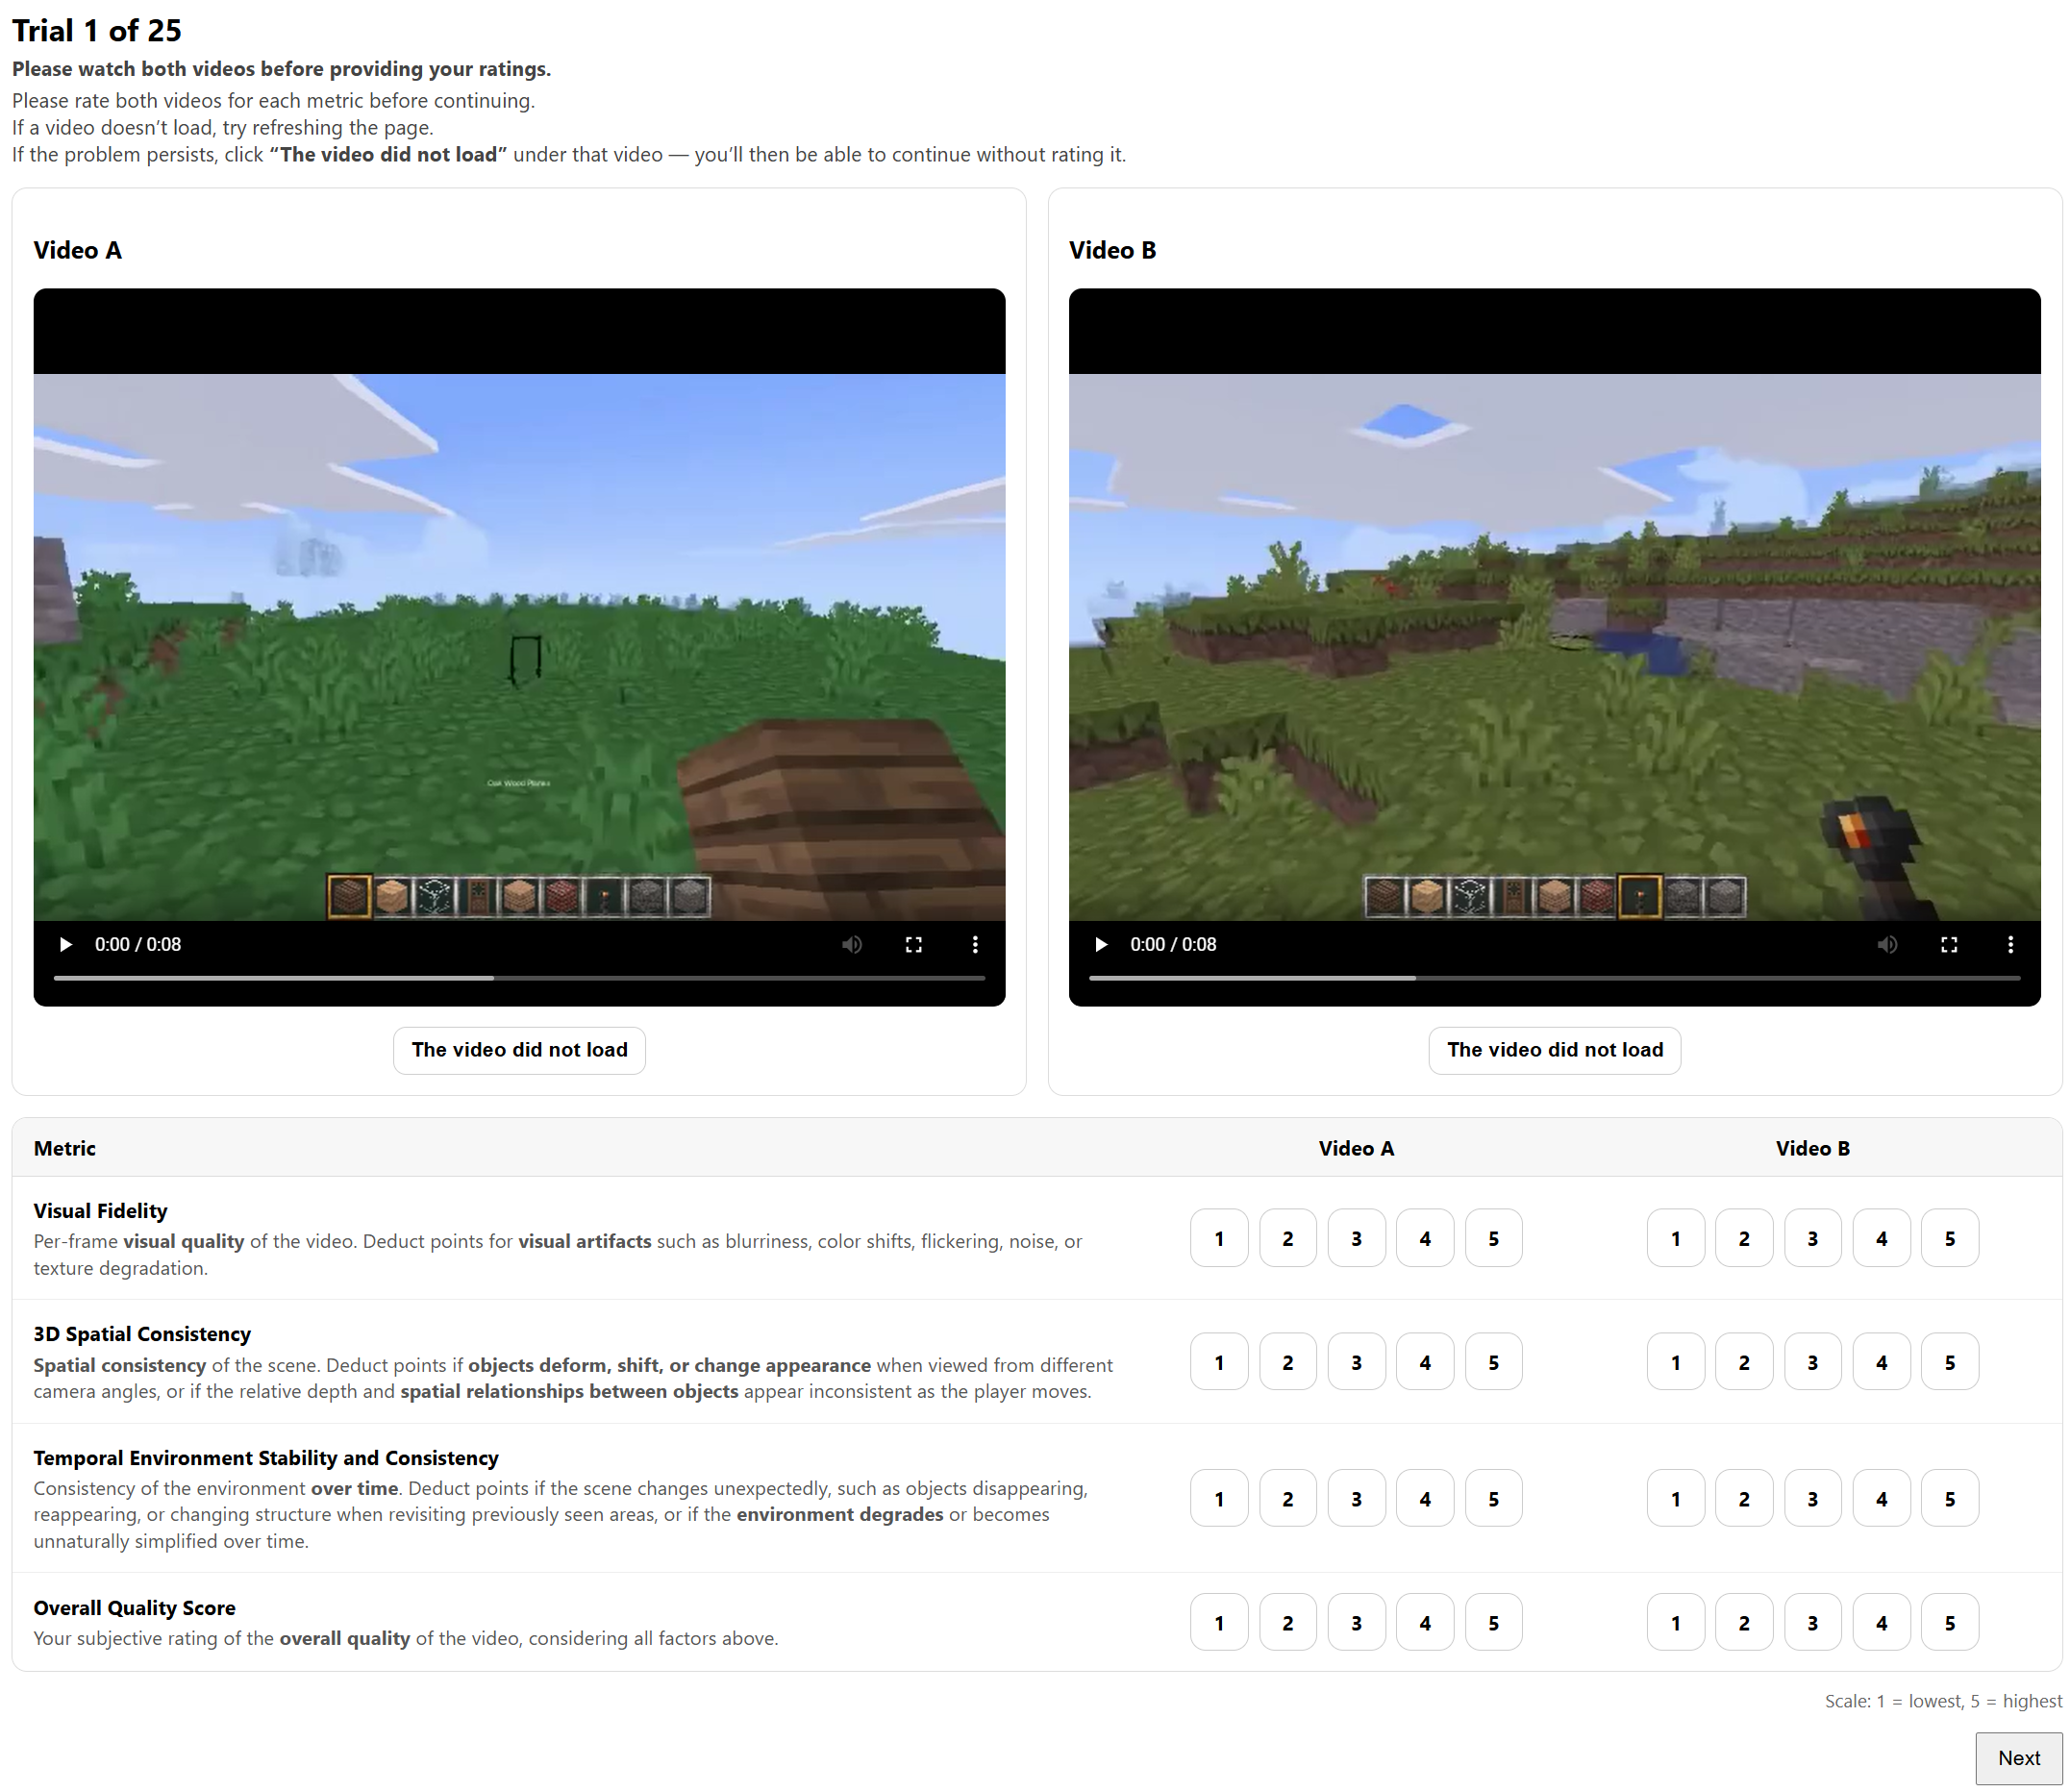
\includegraphics[width=1.0\linewidth]{figs/UI.png}
    \caption{\textbf{User Study Interface.} A screenshot of our web-based platform where participants evaluate video pairs based on temporal and spatial consistency.}
    \label{fig:ui_screenshot}
\end{figure}

%%%%%%%%%%%%%%%%%%%%%%%%%%%%%%%%%%%%%%%%%%%%%%%%%%%%%%%%%%%%%%%%%%%%%%%%%%%%%%%
%%%%%%%%%%%%%%%%%%%%%%%%%%%%%%%%%%%%%%%%%%%%%%%%%%%%%%%%%%%%%%%%%%%%%%%%%%%%%%%

\end{document}

% This document was modified from the file originally made available by
% Pat Langley and Andrea Danyluk for ICML-2K. This version was created
% by Iain Murray in 2018, and modified by Alexandre Bouchard in
% 2019 and 2021 and by Csaba Szepesvari, Gang Niu and Sivan Sabato in 2022.
% Modified again in 2023 and 2024 by Sivan Sabato and Jonathan Scarlett.
% Previous contributors include Dan Roy, Lise Getoor and Tobias
% Scheffer, which was slightly modified from the 2010 version by
% Thorsten Joachims & Johannes Fuernkranz, slightly modified from the
% 2009 version by Kiri Wagstaff and Sam Roweis's 2008 version, which is
% slightly modified from Prasad Tadepalli's 2007 version which is a
% lightly changed version of the previous year's version by Andrew
% Moore, which was in turn edited from those of Kristian Kersting and
% Codrina Lauth. Alex Smola contributed to the algorithmic style files.
